\chapter{Introduction}

\epigraph{``And now you're asking, I don't know where to begin''}{{\sl Mike Vennart, Silent/Transparent}}
%
%“We demand rigidly defined areas of doubt and uncertainty!” 
%― Douglas Adams, The Hitchhiker's Guide to the Galaxy

The release of gravitational potential energy as mass falls towards
a compact object is the most efficient energetic process in the universe,
even more efficient than nuclear fusion.
This {\em accretion} process is thought to power the huge radiative engines at the 
centres of many galaxies -- accreting supermassive black holes 
known as active galactic nuclei (AGN).
As the matter falls into the potential well of the 
black hole it often forms an accretion disc.
This disc is an efficient radiator of the gravitational potential energy released.
and can sometimes outshine the entire stellar population of the galaxy,
appearing as a quasi-stellar object (QSO) or {\em quasar}. 
As well as powering, AGN, 
accretion discs are present in X-ray binaries (XRBs), young-stellar objects (YSOs) and
cataclysmic variables (CVs). Accretion is a universal process; 
broadly speaking, the physics is similar regardless of 
whether matter is falling on to a $\sim1~M_\odot$ neutron star or white dwarf,
or a $\sim10^{10}~M_\odot$ black hole. 

Outflows are ubiquitous in accreting systems. We see collimated radio jets in AGN 
\citep{hazard1963,potash1980,perley1984,marscher2006} and XRBs \citep{bellonijet2010}, 
and there is even evidence of radio emission in 
CVs \citep{benz1983,coppejans2015}. 
These radio jets tend to appear in specific 
accretion states \citep{fender2001,fender2004,kordingDNjet2008}, 
implying an intrinsic connection to the 
accretion process. Even more intriguing, in XRBs less collimated, mass-loaded outflows
or {\em winds} are observed in the opposite accretion state, possibly emanating from the accretion disc.
Evidence for disc winds is widespread across the mass range, but perhaps the most spectacular indication
is the blue-shifted, broad absorption lines (BALs) in the rest-frame ultraviolet (UV)
seen in high-state CVs \citep{heap1978,greensteinoke1982,cordova1982}
and the so-called broad absorption line quasars (BALQSOs) that make up $20-40\%$
of quasars \citep{weymann1991,knigge2008,allen2011}. 
BALs and `P-Cygni' profiles \citep{struve1935,rottenburg1952}
are also seen in stellar winds \citep[e.g.][]{cassinelli1979} and sometimes even
in the optical spectra of CVs \citep{patterson1996, RN98, kafka2004}. 
Broad, blue-shifted absorption is also observed in the Fe K$\alpha$ line in 
some AGN \citep{reeves2003,poundsreeves2009,tombesi2010a} -- these are known
as ultra-fast outflows or UFOs.
% \footnote{It should be noted that, while X-ray spectral
% fitting can be somewhat of a dark art, the explanations for these
% UFOs are somewhat more believable than their sci-fi namesakes.}

The astrophysical significance of disc winds extends, quite literally, 
far beyond the accretion environment. They offer a potential mechanism by which the central
accretion engine can interact with the host galaxy and interstellar medium 
via a `feedback' mechanism \citep{king2003,fabian2012}. 
Feedback is required in models of galaxy evolution \citep{springel2005}
and may explain the famous `$M_{BH}-\sigma$' \citep{silkrees1998,haring2004}
and `$M_{BH}-M_{bulge}$' \citep{magorrian1998} relations.
Winds also offer a natural way to {\em unify} much
of the diverse phenomenology of AGN, CVs and XRBs. This principle of unification
can be applied along more than one `axis' of parameter space. For example, 
there exist elegant models that attempt to explain {\em all}
of the behaviour of quasars with only a central black hole, a jet, an accretion disc,
and an associated outflow, just by varying the viewing angle \citep{elvis2000}.
Similarly elegantly, it has been shown that much of the behaviour of XRBs
is directly applicable to AGN \citep{mchardy2006}, 
and models of outflows in CVs have been successfully `scaled-up'
and applied to quasars and AGN \citep[e.g.][]{higginbottom2013}.

Despite their clear importance and ubiquity, there are still
many unanswered questions relating to the true impact of winds and their underlying
physical origins. Here, I aim to address some of these questions, and 
take steps towards building a more holistic picture of the impact
of winds on the spectral appearance and accretion physics of disc systems.
This thesis is structured as follows. In the remainder of this chapter, 
I will give the background accretion theory 
and detail the successes and failures of accretion 
disc models when compared to observations,
as well as describing the different classes of accreting objects in more detail. 
In chapter 2, I dedicate some time to specifically discussing the theory of,
and observational evidence for, accretion disc winds. In chapter 3, I outline 
the Monte Carlo radiative transfer (MCRT) and photoionization
methods I have used in order to investigate the impact of disc 
winds on the spectra of accreting systems. The next three chapters
contain three separate submitted papers, in which I discuss the impact
of disc winds on the spectra of CVs (Chapter 4), and test disc wind
quasar unification models (Chapters 5 and 6).
In chapter 8, I summarise my findings and their astrophysical significance, 
and discuss potential avenues for future work.


\section{The Physics of Accretion}

The basic phenomenon of accretion- matter falling into a gravitational potential well- 
is ubiquitous in astrophysics. The energy, $\Delta E$, released by a parcel of 
mass, $\Delta m$, falling from infinity onto an object of mass $M$ and radius $R_*$
is given by
\begin{equation}
\Delta E = \frac{GM \Delta m}{R_*},
\label{eq:acc_energy}
\end{equation} 
meaning that the power by mass accreting at a rate $\dot{M}$ is given by
\begin{equation}
L_{acc} = \frac{GM \dot{M}}{R}.
\label{eq:acc_energy}
\end{equation} 
We can also characterise the efficiency of any energetic process by relating
the energy released to the rest mass energy of the parcel of mass, such that
\begin{equation}
\Delta E = \eta \Delta M c^2,
\label{eq:restmass}
\end{equation} 
where $\eta$ is the radiative efficiency. Similarly, in terms of luminosity, $L$,
\begin{equation}
L = \eta \dot{M} c^2,
\label{eq:restmass}
\end{equation} 
Nuclear fusion is one of the more efficient
energetic processes in the universe, with an efficiency of
$\eta=0.007$. If we rearrange the above equations in terms of $\eta$ we find
\begin{equation}
\eta = \frac{G}{c^2} \frac{M}{R_*}.
\label{eq:eta}
\end{equation} 
In other words, the efficiency of accretion is directly related 
to the {\em compactness}, $M/R_*$, of the central object. 
% Values of compactness for four different compact objects
% are shown in table~\ref{compactness}. 

\subsection{Spherical Accretion and The Eddington Limit}
\label{sec:eddington}

The simplest geometry one might propose for accretion
would be one in which a central mass accretes matter from
an all-encompassing cloud.
The process of spherical accretion has come to be known as 
Bondi-Hoyle-Lyttleton accretion \citep{hoyle1939,bondi1944}.
In particular, \cite{bondi1952} studied spherically symmetric 
accretion onto a point mass and derived the Bondi radius,
\begin{equation}
r_B = \frac{G M}{c_S^2},
\label{eq:bondi}
\end{equation} 
where $c_S = c_S(r_B)$ is the sound speed as a function of radius.
The Bondi radius represents a critical point inside which the material
is supersonic and will accrete on the free-fall timescale.

When this timescale is long enough, the accreting matter
can radiate away its potential energy, generating a luminosity $L$. 
This radiation will induce a force on electrons, given by
\begin{equation}
F_{rad} = \frac{L \sigma_T}{4 \pi r^2 c},
\label{eq:frad}
\end{equation} 
where $\sigma_T = 6.65\times10^{-25}$cm$^2$ is the Thomson cross-section.
If this radiation force term dominates over the gravitational
force, then the material will no longer fall inwards. Consider
radiation pressure acting on electron-proton pairs, for which the gravitational
force is approximately given by $G M m_p / r^2$. Combining this expression
with equation~\ref{eq:frad} gives a natural
maximum accretion luminosity, known as the {\em Eddington limit}, of
\begin{equation}
L_{Edd} = \frac{4 \pi G M m_p c}{\sigma_T},
\label{eq:bondi}
\end{equation} 
with an associated Eddington accretion rate of 
\begin{equation}
\dot{M}_{Edd} = \frac{L_{Edd}}{\eta c^2}.
\label{eq:bondi}
\end{equation} 
The Eddington limit makes a number of assumptions, namely
that the accretion flow is steady, spherically symmetric, ionized,
and has its opacities dominated by electron scattering.
Clearly, there are many astrophysical situations where this does not hold.
For example, the recent outburst of V404 Cyg showed wildly variable
luminosities on short timescales 
\citep[see, e.g.,][among many, many ATels]{kuulkers_atel2015,motta_atel2015}, 
and in any binary system
or disc dominated system the assumption of spherical symmetry will
break down. Nevertheless, the Eddington limit provides a good order of magnitude 
estimate of the maximum luminosity of an accreting object,
and also provides a useful way of parameterising accretion rate,
as it scales linearly with mass. It can also be used
to characterise the {\em state} of an accretion disc.  
In general, sources above $\sim 0.1~L_{Edd}$ find themselves in a 
`soft' or thin-disc state, whereas for much lower Eddington 
fractions, sources will possess advection-dominated accretion flows
\citep[ADAFs; ][]{narayan1994,narayan1995}.
It is also clear that around the Eddington limit radiation pressure
must play a major role in determining the disc morphology 
(see section~\ref{sec:rad_winds}).

\subsection{Accretion Discs}

In many astrophysical situations -- for example, 
in binary systems and gas clouds orbiting BHs --
any accreting matter will possess some net angular momentum.
If the medium is dense enough, collisions between particles will be
frequent, but the total angular momentum vector of two colliding particles
will always be conserved. This provides a mechanism for a gas cloud to relax to 
its minimum energy state -- an accretion disc. 

As well as losing gravitational potential energy as it falls towards 
the central mass, a parcel of matter must also lose its angular momentum. 
Crucially, accretion discs provide a way for this to happen. 
If the disc overall maintains the same total 
angular momentum, it follows that angular momentum must 
therefore be transported outwards. The mechanism for transporting 
angular momentum outwards is unknown, and is one of the biggest 
weaknesses of current accretion disc theory. The most commonly invoked
candidate is the magnetorotational instability \citep[MRI; ][]{balbus1991},
in which accretion discs are subject to a strong shearing instability even
when the magnetic field is weak. Possible alternative are
that the angular momentum is lost
via a a magnetohydrodynamic outflow \citep{blandfordpayne} or spiral shock waves
\citep{ju2016}. An efficient mechanism
for angular momentum transport is necessary as the 
viscosity introduced in the next section is
generally inefficient in this regard \citep{pringle1991}.


% \begin{table}
% \centering
% \begin{tabular}{p{2cm}p{2cm}p{2cm}p{2cm}}
% \hline Object & $M (M_\odot)$ & $R$ (cm) & $\eta$ \\ 
% \hline \hline 
% White Dwarf & $0.8$ & $7\times10^{8}$
% Neutron Star & $1.4$ & 
% Black Hole & $10$ & 
% SMBH & $10^9$ & $8.85\times10^{14}$
% \end{tabular}
% \centering
% \caption{
% Values of compactness for four different compact objects.
% }
% \label{wind_param}
% \label{modelb_table}
% \end{table}



\subsubsection{Steady-state Accretion Discs: The $\alpha$-prescription}

\label{sec:alpha_disc}

The so-called $\alpha$-disc model developed by 
\citet[][hereafter SS73]{shakurasunyaev1973} and \cite{lyndenbell1969} is
currently the leading candidate for explaining how energy and angular momentum
is transported an accretion disc. 
The starting point for this model is the parameterisation
of viscosity, $\nu^\prime$, using the simple form
\begin{equation}
\nu^\prime = \alpha c_s H,
\label{eq:viscosity}
\end{equation}
where $H$ is the scale height of the disc,
$\alpha$ is a parameter $\leq 1$ and $c_s$ is the sound speed.
Viscous torques then allow the conversion of orbital kinetic energy into heat, 
which can be radiated away. 
If we make one further assumption, that the accretion rate is
constant throughout the disc, we can write down a mass continuity equation
valid at all radii, given by
\begin{equation}
\dot{M} \equiv 2 \pi R V_R \Sigma = 0,
\end{equation}
where $\Sigma$ is the surface density at that point. 
The angular momentum equation then becomes
\begin{equation}
\nu^\prime \Sigma = \frac{\dot{M}}{3 \pi} \left[1 - \left( \frac{R}{R_*} \right)^{1/2} \right]\, .
\label{eq:viscous_angmom}
\end{equation}
The viscous torques throughout the disc cause a local loss of mechanical energy, allowing 
one to derive \citep[see, e.g.][]{fkrbook} a rate of viscous dissipation, per unit area, given by
\begin{equation}
D(R) = \frac{1}{2} \nu^\prime \Sigma (R \Omega^\prime)^2.
\label{eq:dissipation1}
\end{equation}
Here, $D(R)$ is proportional to the derivative of the angular velocity, $\Omega^\prime=d\Omega/dR$.
By combining equations~\ref{eq:dissipation1} and \ref{eq:viscous_angmom} we can show that the 
viscous dissipation rate is 
\begin{equation}
D(R) = \frac{G M \dot{M}}{8 \pi R^3} \left[1 - \left( \frac{R}{R_*} \right)^{1/2} \right]
\label{eq:dissipation2}
\end{equation}
where we have also set the angular velocity to the Keplerian velocity. 
This expression is independent of viscosity -- which is fortunate, because
we do not know what value of $\alpha$ to use in equation~\ref{eq:viscosity}.
This result comes about because of the implicit assumption that the viscosity regulates
the mass accretion rate so as to achieve a steady state.

We can now integrate across both sides of the whole disc to obtain the disc luminosity,
\begin{equation}
L_{disc} = 2 \int^\infty_{R_*} D(R) 2\pi R dR = \frac{G M \dot{M}}{2 R_*} = \frac{1}{2} L_{acc}\, .
\label{eq:ldisc}
\end{equation}
This result can also be shown by considering the binding energy of gas at $R_*$ and infinity.
From equation~\ref{eq:dissipation2} one can also derive an effective temperature distribution,
by setting
\begin{equation}
\sigma T_{eff}^4 (R) = D(R),
\end{equation}
which then gives
\begin{equation}
T_{eff} (R) = T_* \left[1 - \left( \frac{R}{R_*} \right)^{1/2} \right]^{1/4},
\label{disk_t_profile}
\end{equation}
where
\begin{equation}
T_* = \left ( \frac{3 G M \dot{M}}{8 \pi R_*^3 \sigma} \right)^{1/4}.
\end{equation}
When $R>>R_*$ this simplifies to
\begin{equation}
T_{eff} (R) = T_* (R / R_*)^{-3/4}.
\end{equation}
Now we have not only derived the total luminosity of an accretion disc, but
also the effective temperature profile which will govern the shape of the emergent SED.
This temperature profile is shown in figure~\ref{fig:disk_t}
for three different compact objects, assuming an Eddington fraction of 0.2.

\begin{figure}
\centering
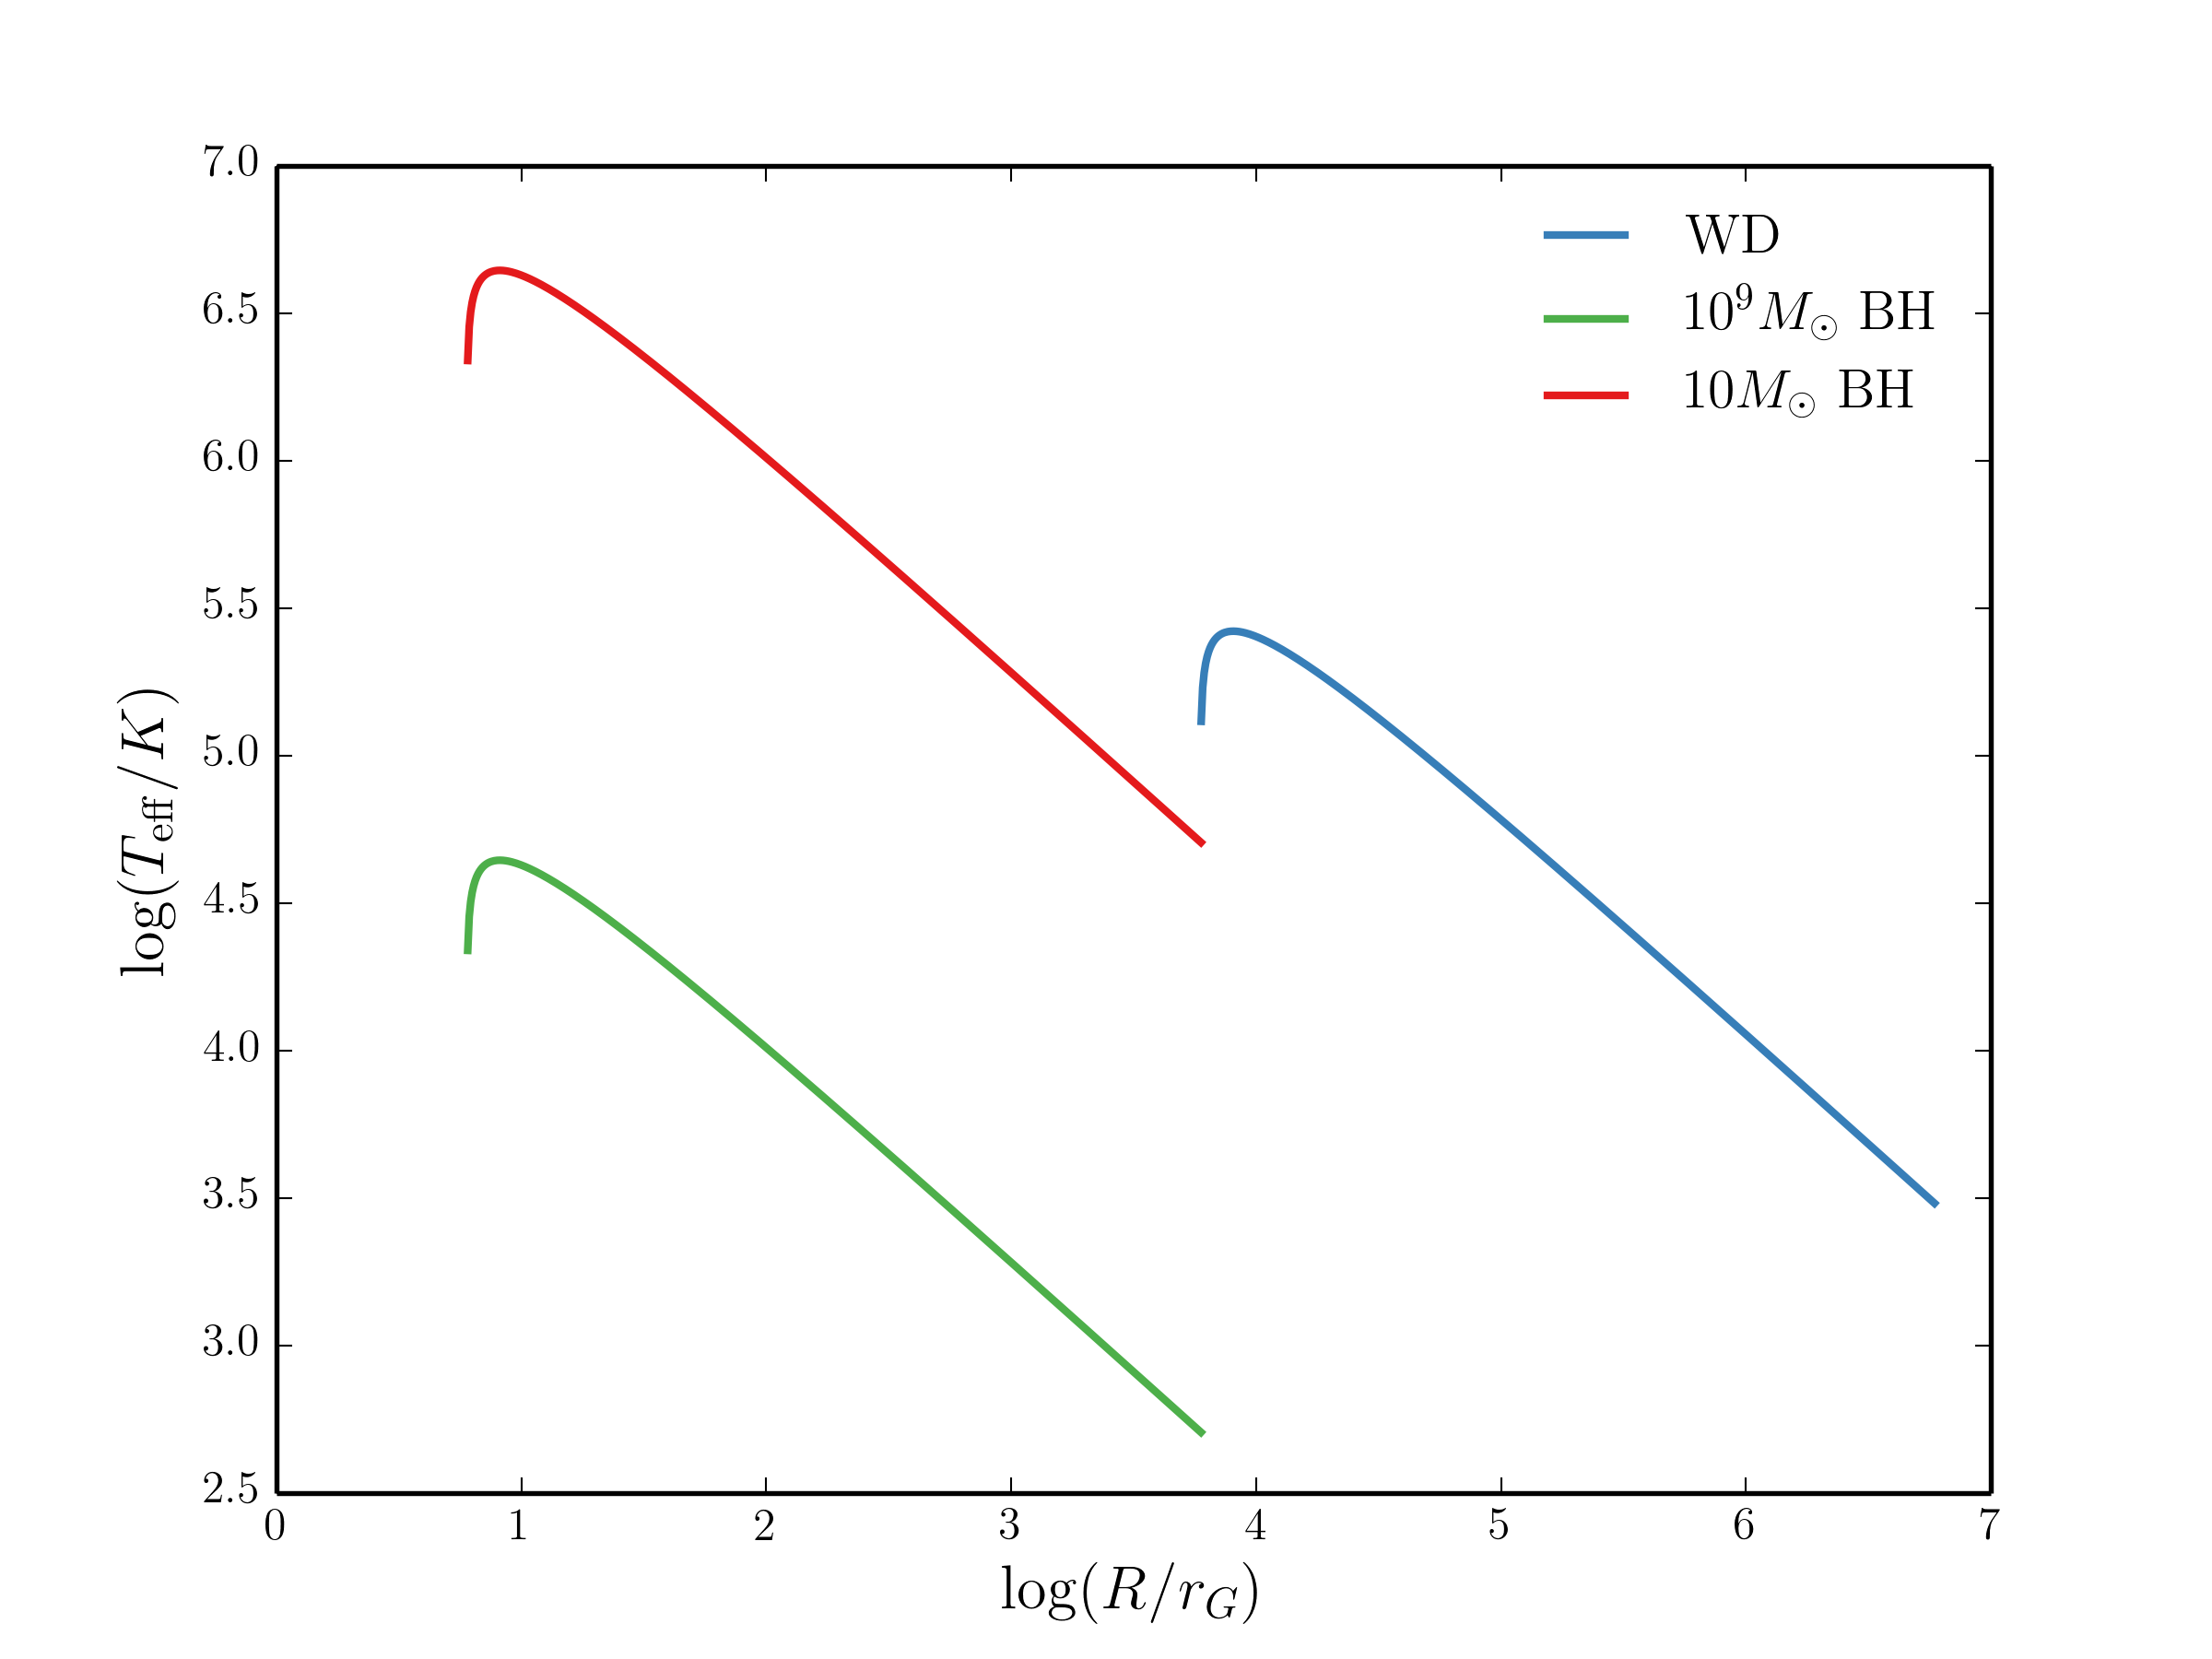
\includegraphics[width=1.0\textwidth]{figures/01-intro/disk_t.png}
\caption
[The temperature profile of an accretion disc for three different classes
of compact object.]
{
The temperature profile of an accretion disc for three different classes
of compact object.
} 
\label{fig:disk_t}
\end{figure}

\subsection{Boundary layers, black hole spin and the ISCO}

In equation~\ref{eq:ldisc} I showed that $L_{disc} = 1/2~L_{acc}$. 
One might then ask: where does the rest of the luminosity go?
The answer is dependent on the compact object in question. 
In an accreting WD, the rotating matter must eventually deposit itself 
on the surface of the WD. This is illustrated in figure~\ref{fig:omega},
which shows the angular velocity as a function of radius in a disc around
a compact object rotating with angular velocity $\Omega_*$. The boundary layer (BL)
is the region to the left of the dotted line, inside the maximum of $\Omega_K$, the Keplerian
angular velocity. The luminosity of the boundary layer is \citep{fkrbook}
\begin{equation}
L_{BL} = \frac{1}{2}\frac{GM \dot{M}}{R} \left[1 - \left(\frac{\Omega_*}{\Omega_K(R_*)}\right)\right]^2,
\end{equation}
where $\Omega_K(R_*)$ is the Keplerian angular velocity at $R_*$, assuming the thickness
of the BL is small. When $\Omega_K(R_*) \gg {\Omega_*}$, this reduces to 
$L_{BL} = 1/2~L_{acc} = L_{disc}$

In cataclysmic variables, 
BLs can be approximated with blackbodies and their temperatures estimated
indirectly via the \cite{zanstra1929} method \citep[e.g.][]{hoare1991,hoaredrew1993}.
However, they likely exhibit a variety of atomic features \citep{suleimanov2014}.
Extreme-UV (EUV) datasets have confirmed the existence of boundary layer emission
in non-magnetic CVs \citep{mauche1996}, although these observations
are limited in number.

\begin{figure}
\centering
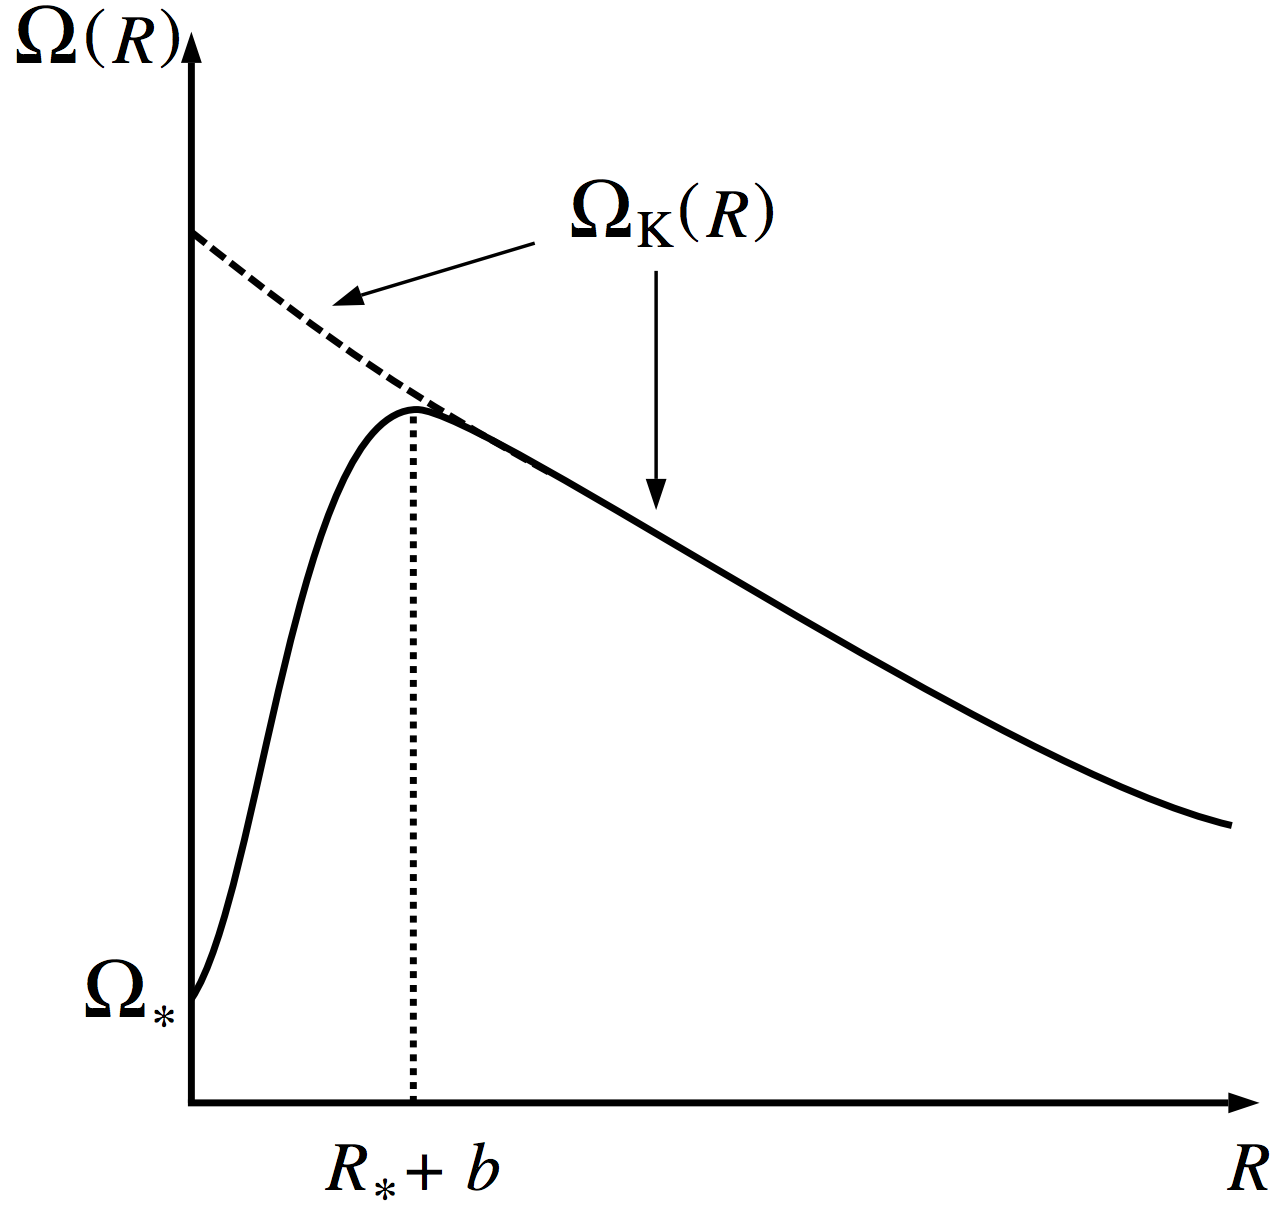
\includegraphics[width=0.7\textwidth]{figures/01-intro/omega.png}
\caption
[Angular velocity as a function of radius in an accretion disc around a rotating
compact object.]
{
{\sl Credit: Frank et al. 2002}.
Angular velocity as a function of radius in an accretion disc around a rotating
compact object with angular velocity $\Omega_*$. $\Omega_K$ is the Keplerian 
angular velocity. This graph
also helps explain why there is a turnover in the temperature-radius relation,
as $D(R)$ is proportional to the square of the {\em derivative} of this quantity.
} 
\label{fig:omega}
\end{figure}

Clearly, in BH systems a boundary layer cannot exist in the same way,
due to the lack of a physical surface. Instead, the energy must either go into
growing the BH, contributing to its angular momentum or being
channeled into a jet or other radiative source (see section~\ref{sec:disc-jet}).
The question of what happens at the inner disc edge
is complicated further by the fact that the disc cannot extend to the 
event horizon of the BH. Instead, there is an `innermost stable circular orbit' (ISCO)
beyond which the accreting matter will simply fall 
into the BH along nearly radial paths. The radius
of this orbit, $R_{ISCO}$, and the horizon radius, $R_H$,
is shown for different values of the BH spin parameter, $a_*$, 
in figure~\ref{fig:isco}, showing how matter can orbit closer to a prograde spinning BH. 
In estimating the luminosity of a Keplerian disc around a BH, 
one should really set $R_* = R_{ISCO}$ in equation~\ref{eq:eta}, giving us the interesting
result that rapidly spinning (Kerr) BHs are more radiatively efficient 
than Schwarzschild BHs.

\nocite{narayan2014, thorne1974}
\begin{figure}
\centering
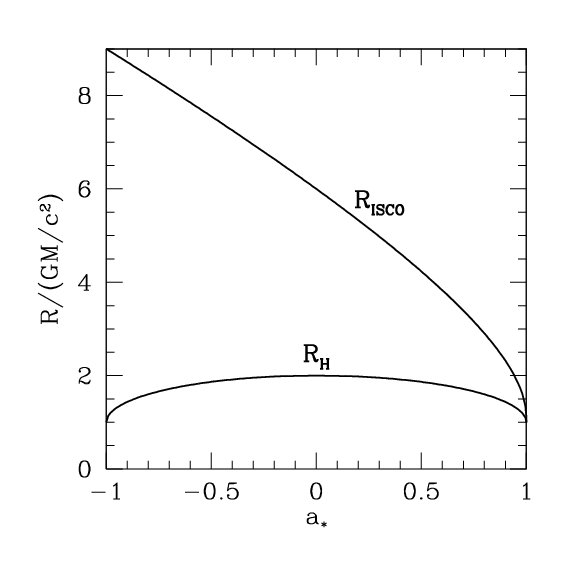
\includegraphics[width=0.7\textwidth]{figures/01-intro/isco.png}
\caption
[The radius of the ISCO, $R_{ISCO}$, and the horizon, $R_H$,
is as a function of the BH spin parameter, $a_*$.]
{
{\sl Credit: Narayan 2014.}
The radius of the ISCO, $R_{ISCO}$, and the horizon, $R_H$,
is as a function of the BH spin parameter, $a_*$. 
$a_*=0$ corresponds to a Schwarzschild BH, and $a_*=1$ and $a_*=-1$
to prograde and retrograde Kerr BHs respectively. Note that
this figure ignores the counteracting torque of photons swallowed by the BH,
which actually limits $a_*$ to a value of around $0.998$ (Thorne 1974).  
} 
\label{fig:isco}
\end{figure}


\subsection{The emergent spectrum}


\begin{figure}
\centering
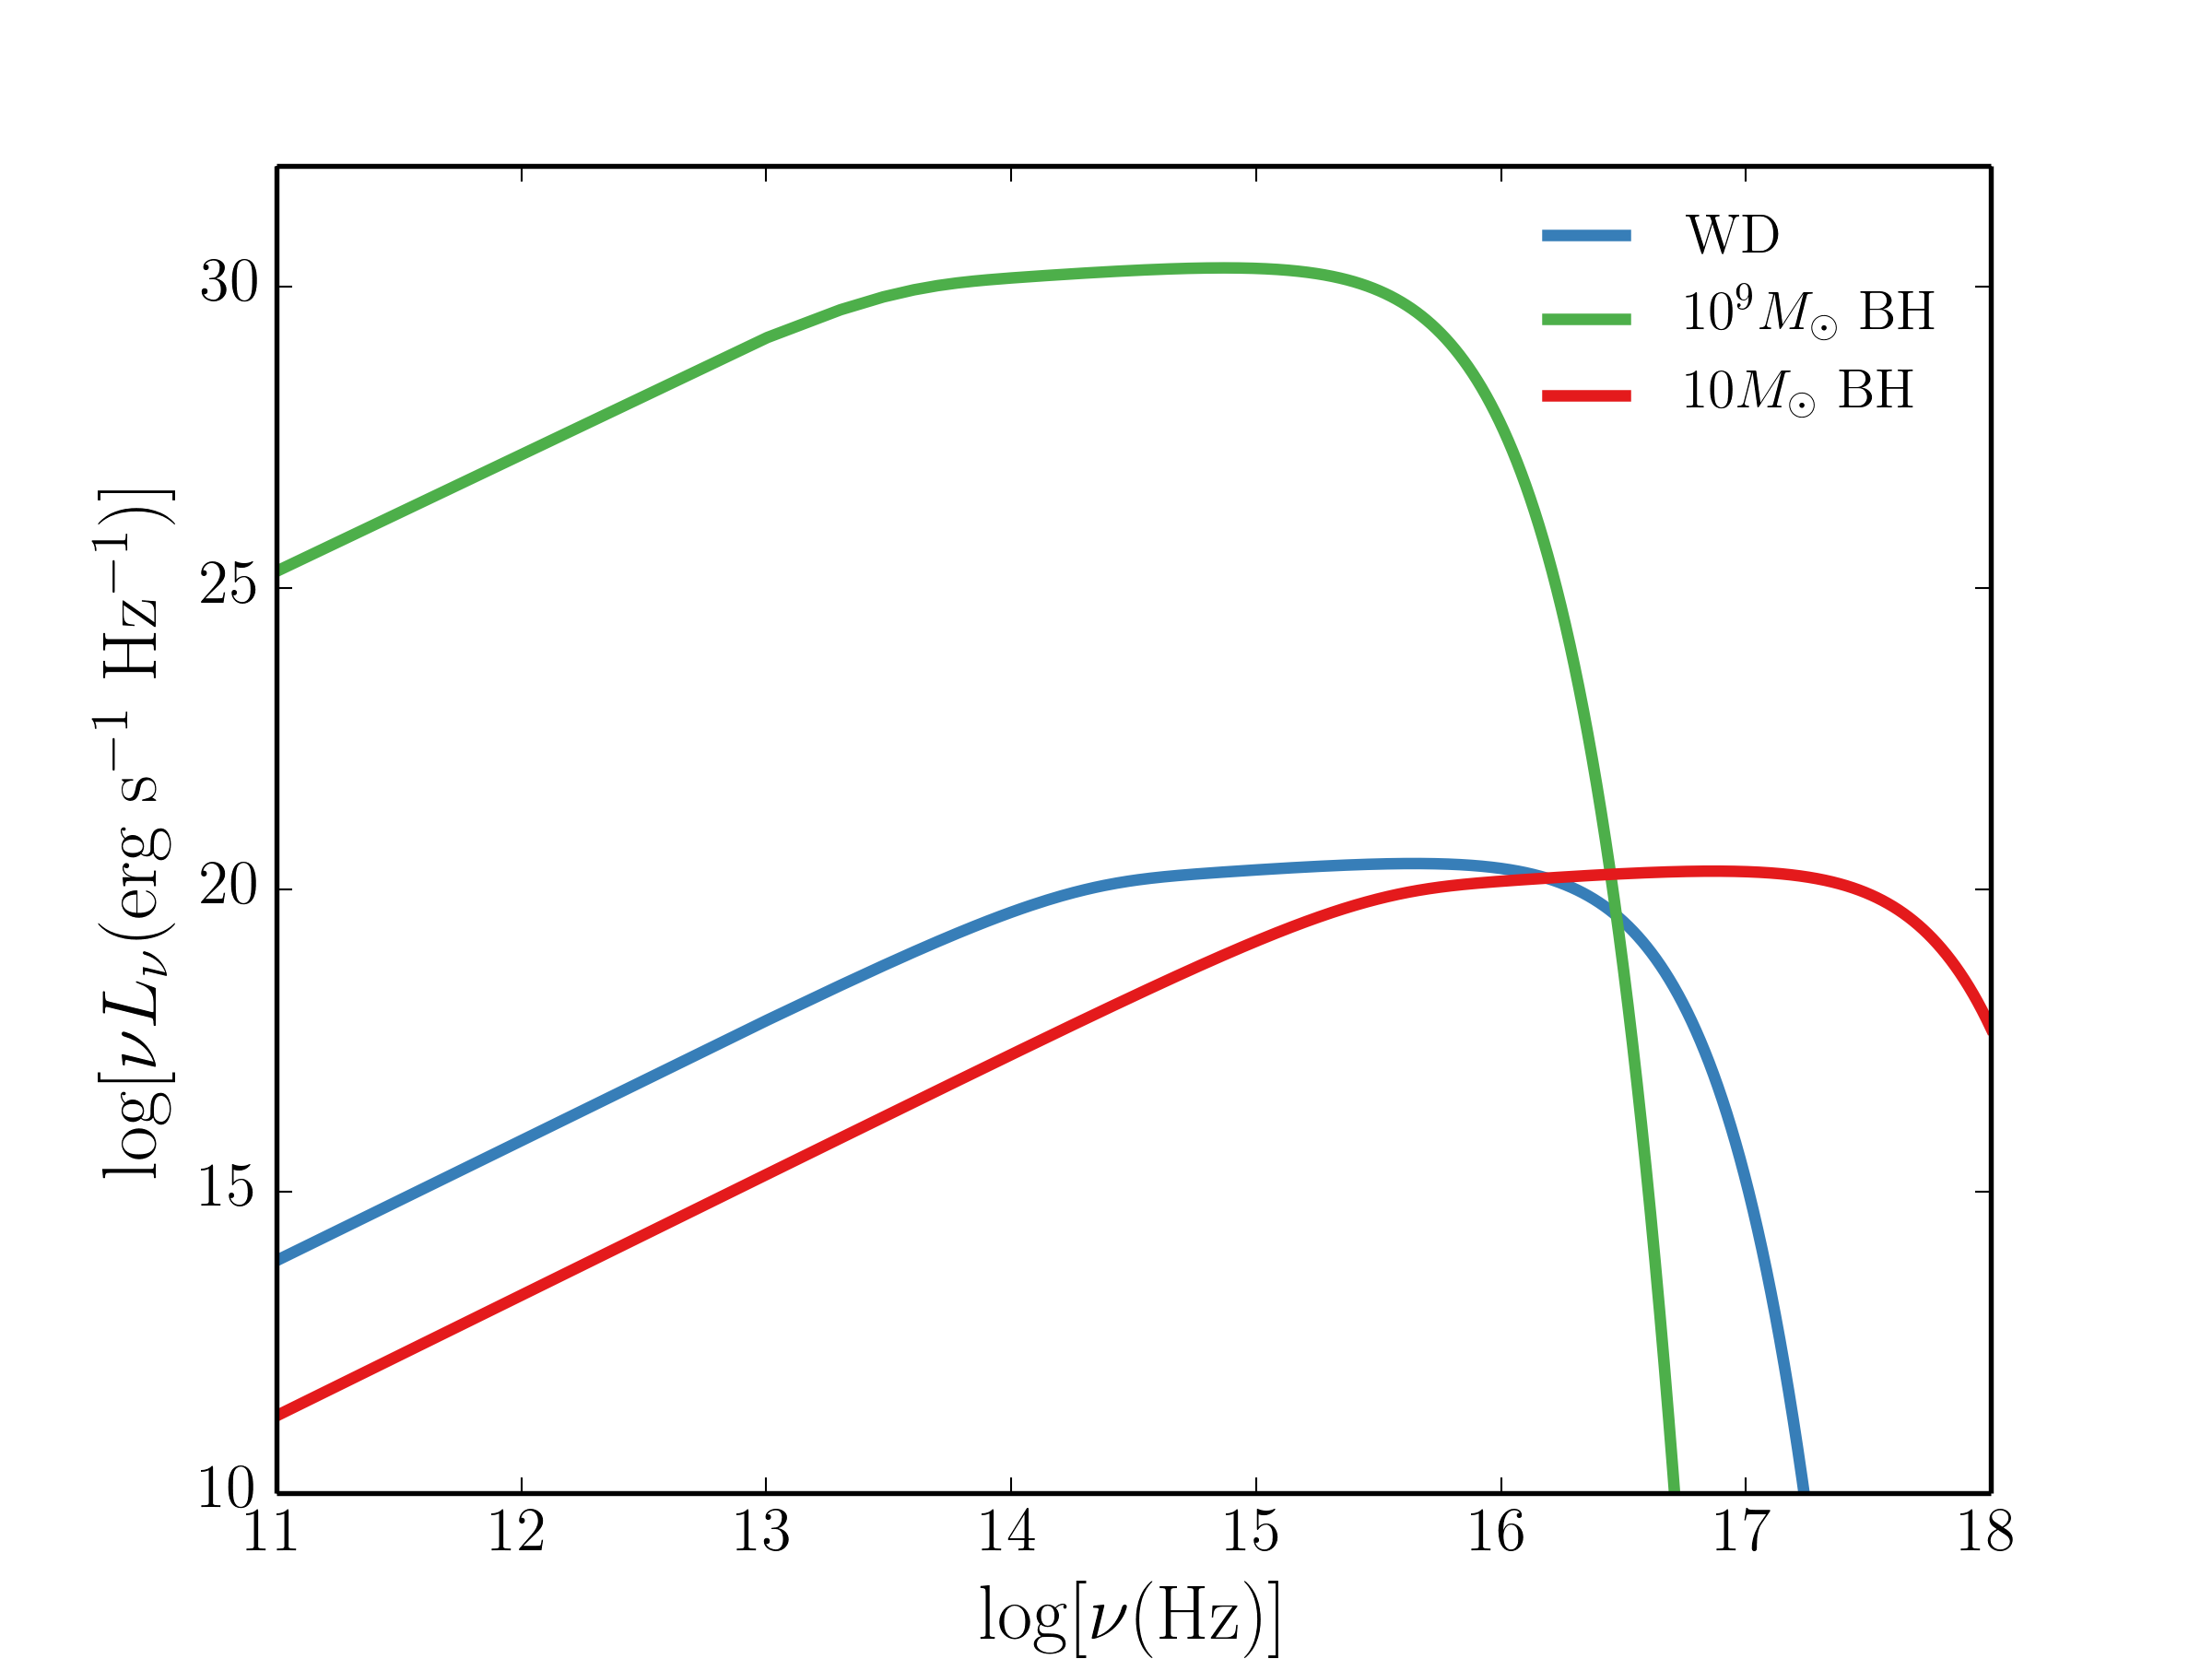
\includegraphics[width=0.8\textwidth]{figures/01-intro/disc_seds.png}
\caption
[Accretion disc SEDs for three different compact objects.]
{
Accretion disc SEDs for three different compact objects, corresponding roughly
to a quasar, an XRB and a CV. The SEDs are computed via an area-weighted sum
of blackbodies with effective temperatures governed by equation~\ref{disk_t_profile},
and the $\nu^{1/3}$ shape in the middle of the spectra can be seen.
} 
\label{fig:disc_seds}
\end{figure}

It is important to recognise that the steady-state disc treatment
{\sl does not specify the exact shape of the disc SED}. What it does do is 
say where energy is originally released. The simplest assumption is
that each annulus emits as a blackbody with temperature 
$T_{eff} (R)$, and the specific intensity through the emitting surface
thus follows the Planck Law:
\begin{equation}
B_\nu (T) = \frac{2 h \nu^3}{c^2} \frac{1}{\exp(h\nu / kT) - 1}
\label{eq:planck}
\end{equation}
Under this assumption it is possible to show that at intermediate frequencies, 
where $kT(R_{max}) \ll h \nu \ll kT_*$,
then the spectrum appears as a `stretched blackbody' with the form 
\begin{equation}
F_{\nu} \propto \nu^{1/3}.
\end{equation}
Figure~\ref{fig:disc_seds} shows the blackbody SEDs expected for the same 
objects as figure~\ref{fig:disk_t}, in
which the $\nu^{1/3}$ portion can be clearly seen.
A disc atmosphere model with frequency-dependent opacity creates a somewhat 
different (and more realistic) spectrum. 
Figure~\ref{fig:bb_v_sa} shows a comparison between a stellar atmosphere model and
blackbody model for $T_{eff}=50,000$K, showing how an annulus at that temperature
can have a significantly different spectral shape when one includes frequency-dependent opacities
in the atmosphere. It is of course possible that {\em neither} blackbody or disc atmosphere
treatments are realistic. I shall therefore devote a little time to discussing
the observational arguments for accretion discs and reviewing
the different classes of accreting objects.

% \begin{figure}
% \centering
% 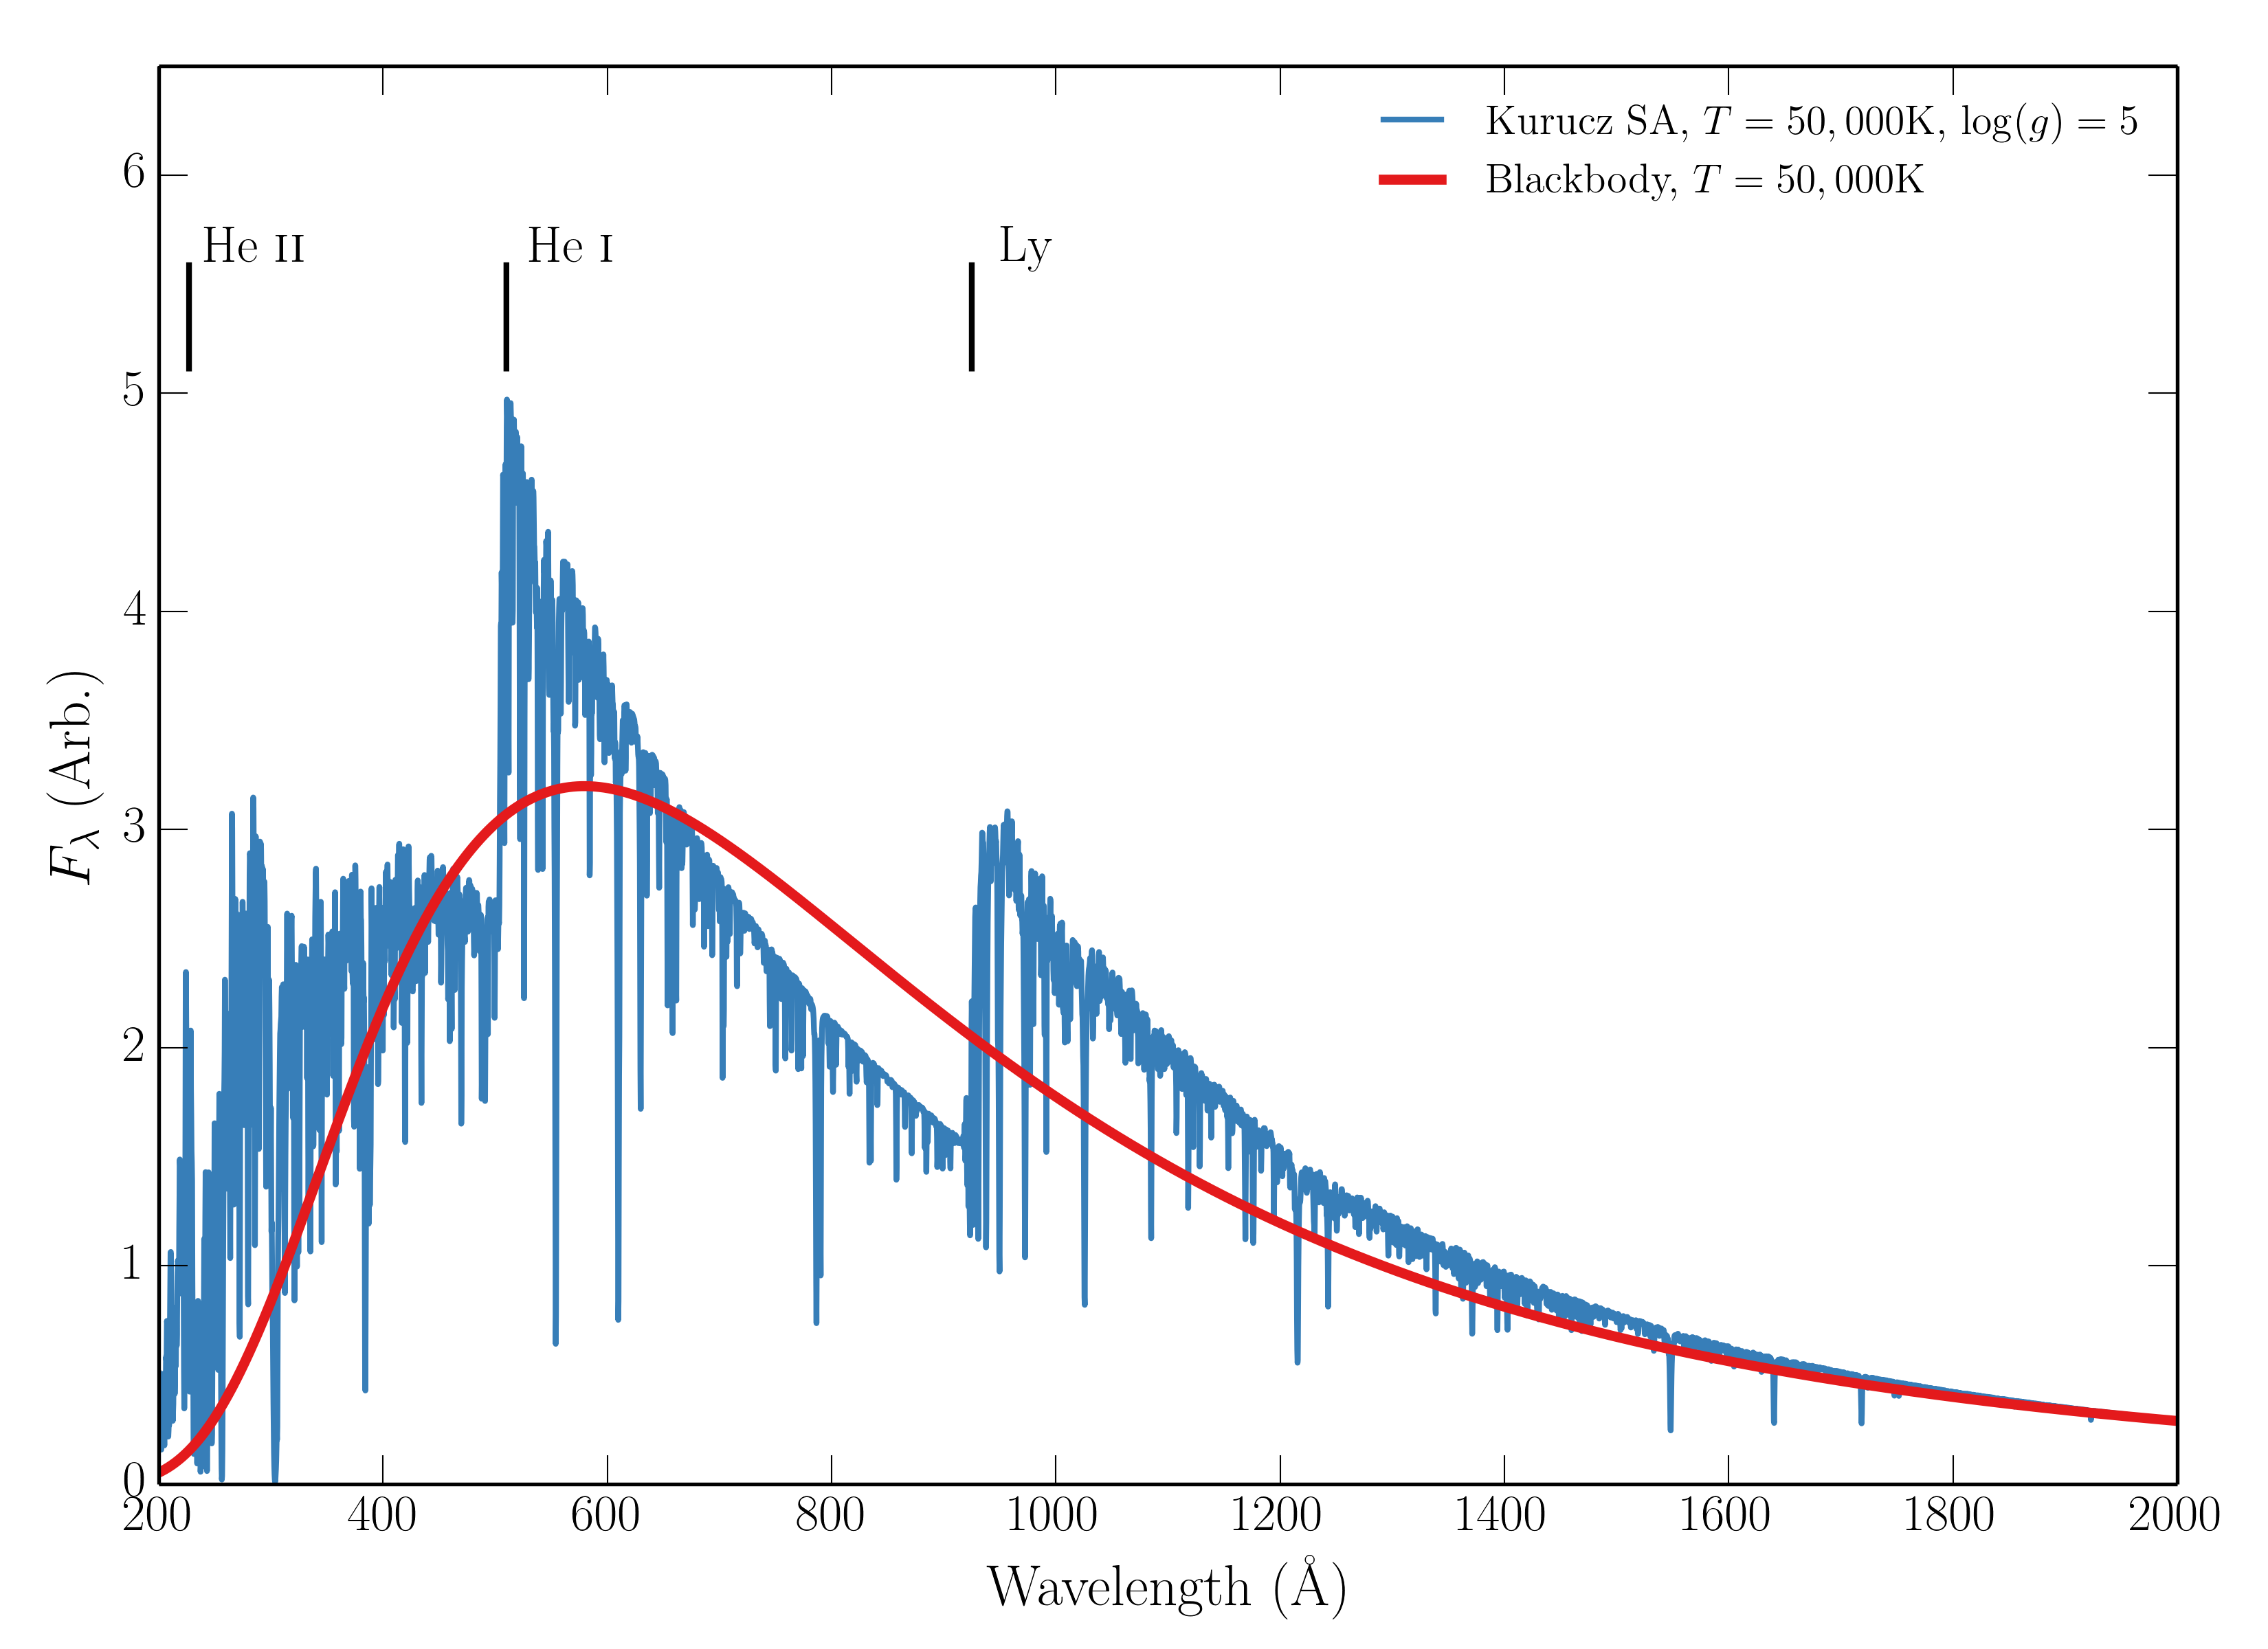
\includegraphics[width=0.8\textwidth]{figures/01-intro/bb_v_sa.png}
% \caption
% [A comparison between a Planck curve and Kurucz (1991) stellar atmosphere model.]
% {
% A comparison between a Planck curve and Kurucz (1991) stellar atmosphere model
% at $T_{eff}=50,000$K and surface gravity of $\log(g)=5$. The major photoabsorption
% edges are marked. Flux is reprocessed into different wavelengths by bound-free opacities,
% and line blanketing also has a big effect on the spectrum. The Hydrogen and Helium lines
% also experience significant pressure broadening.
% } 
% \label{fig:bb_v_sa}
% \end{figure}

\begin{figure}
\centering
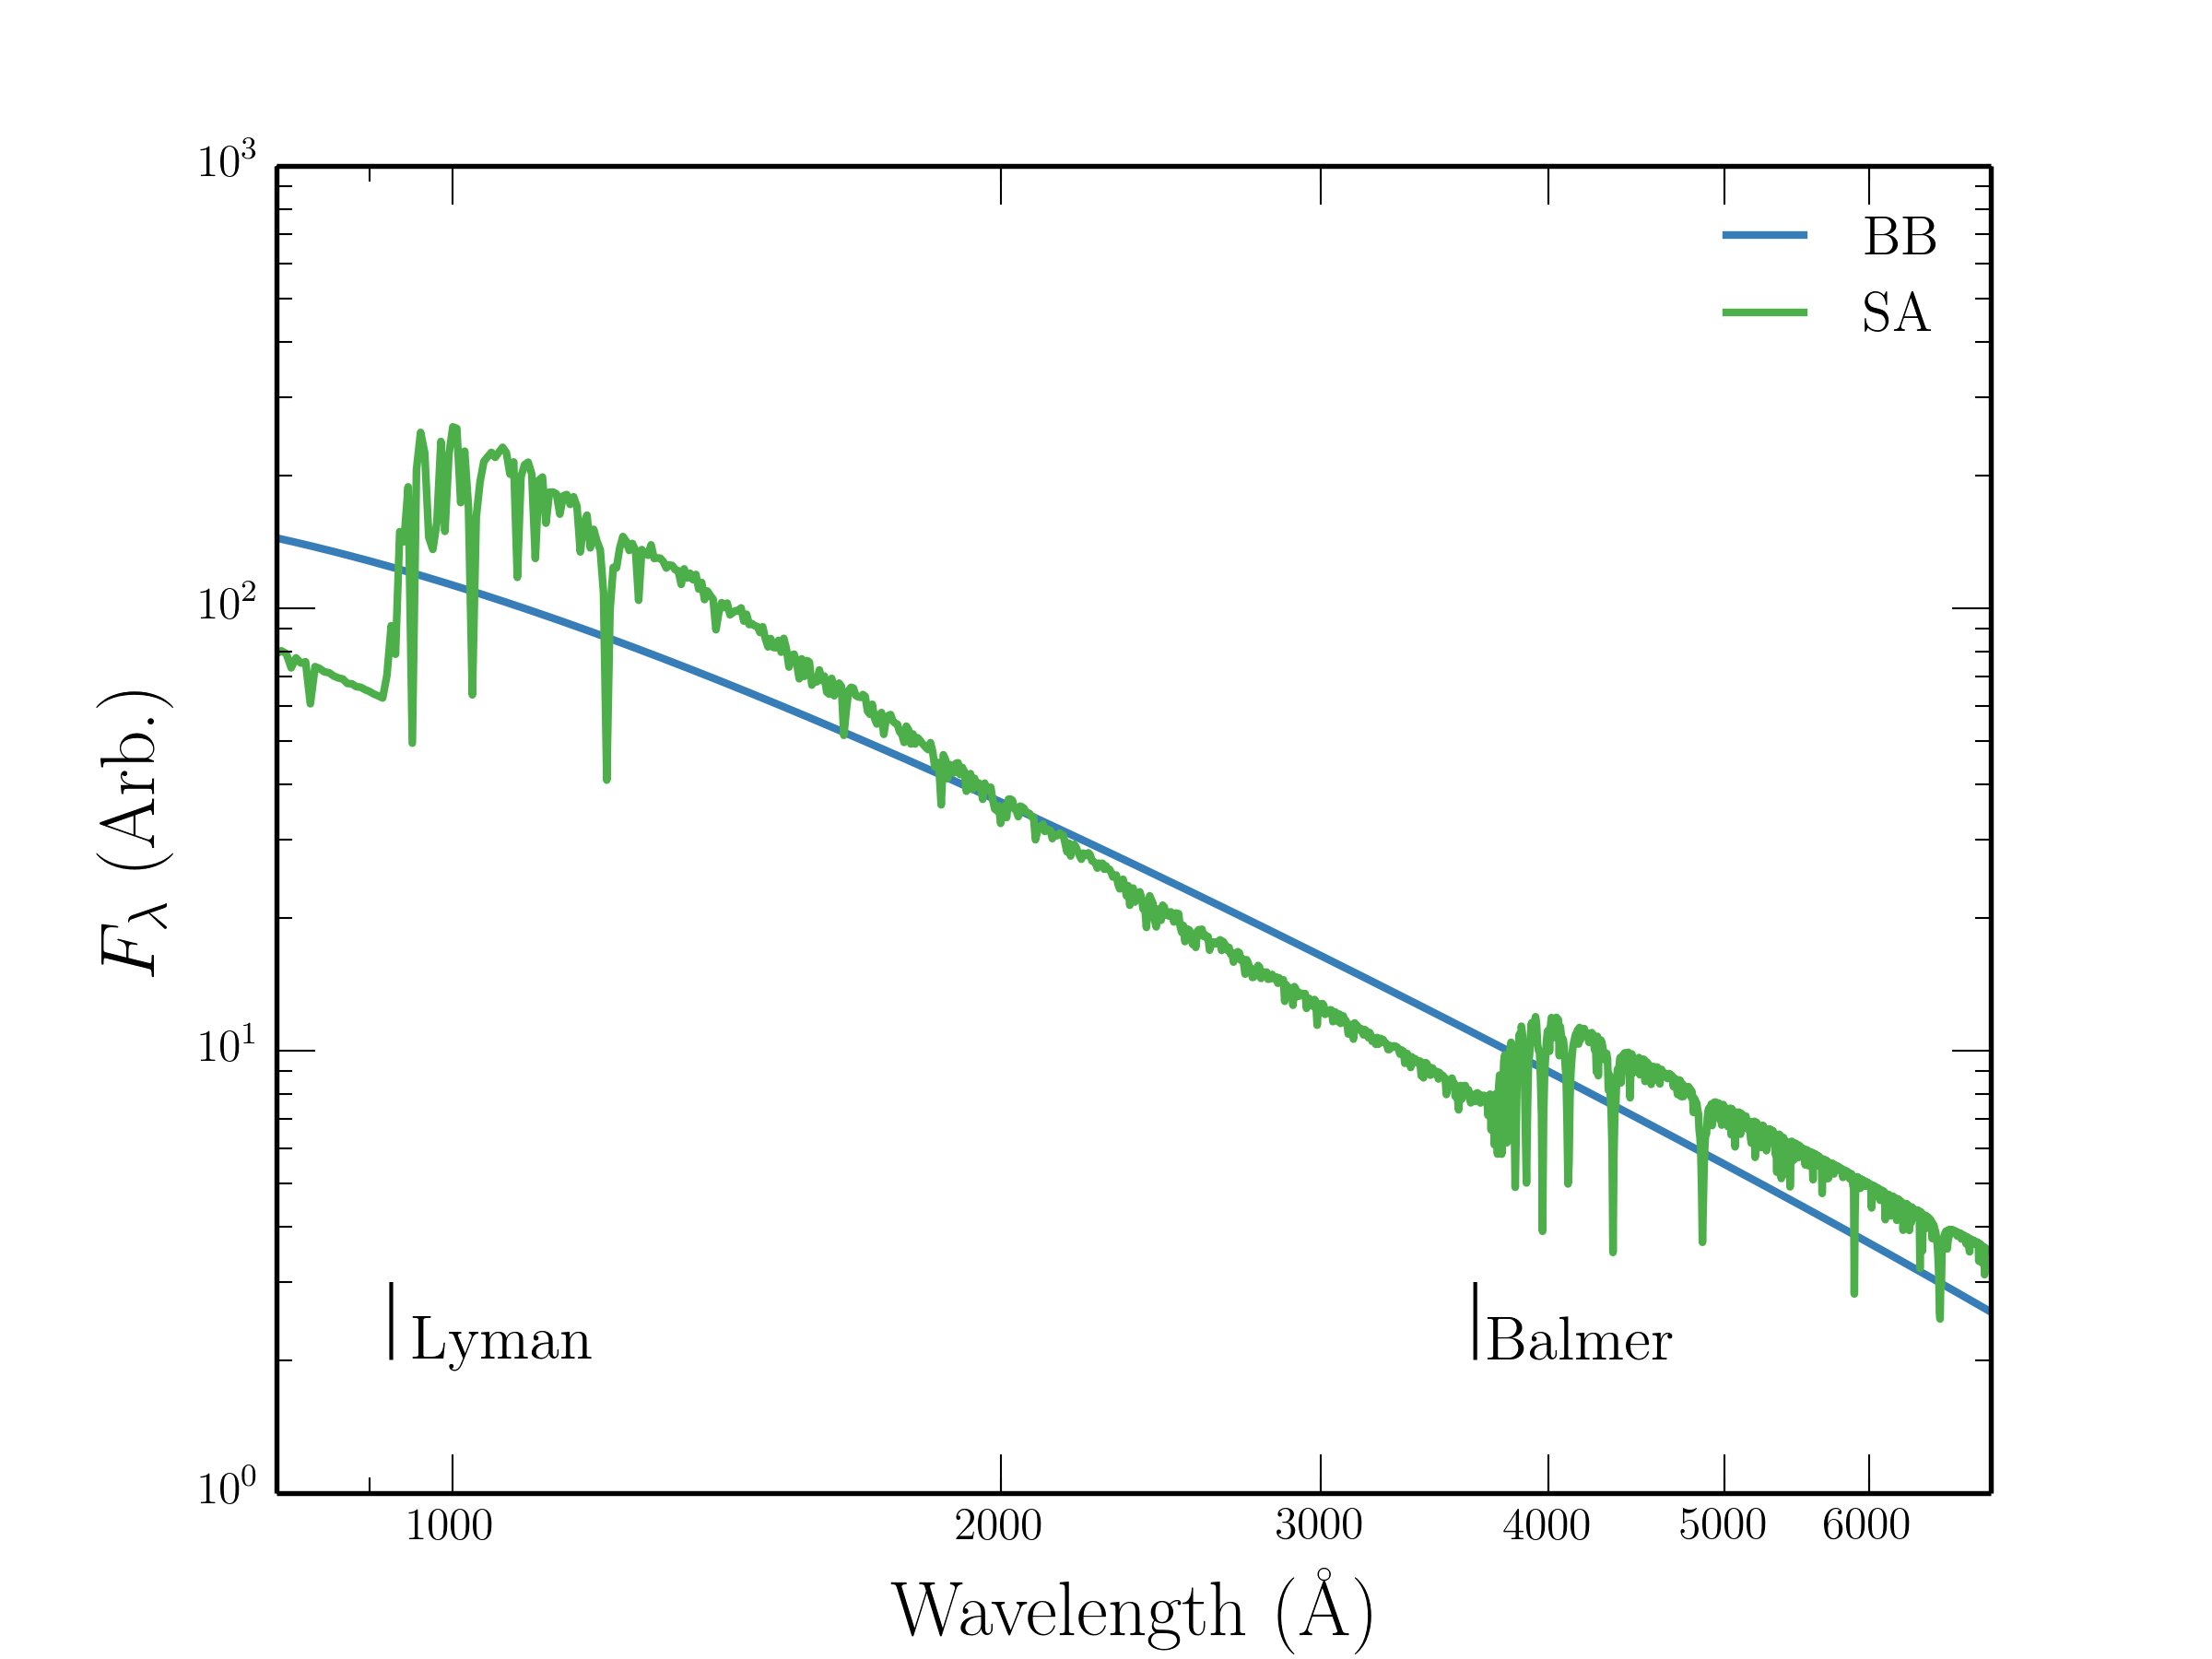
\includegraphics[width=0.8\textwidth]{figures/01-intro/disc_spectrum_comparison.png}
\caption
[A comparison between an accretion disc spectrum computed 
with blackbody and stellar atmosphere spectra.]
{
A comparison between a Planck curve and Kurucz (1991) stellar atmosphere model
at $T_{eff}=50,000$K and surface gravity of $\log(g)=5$. The major photoabsorption
edges are marked. Flux is reprocessed into different wavelengths by bound-free opacities,
and line blanketing also has a big effect on the spectrum. The Hydrogen and Helium lines
also experience significant pressure broadening.
} 
\label{fig:bb_v_sa}
\end{figure}



\section{Accreting Compact Binaries}

\begin{figure}
\centering
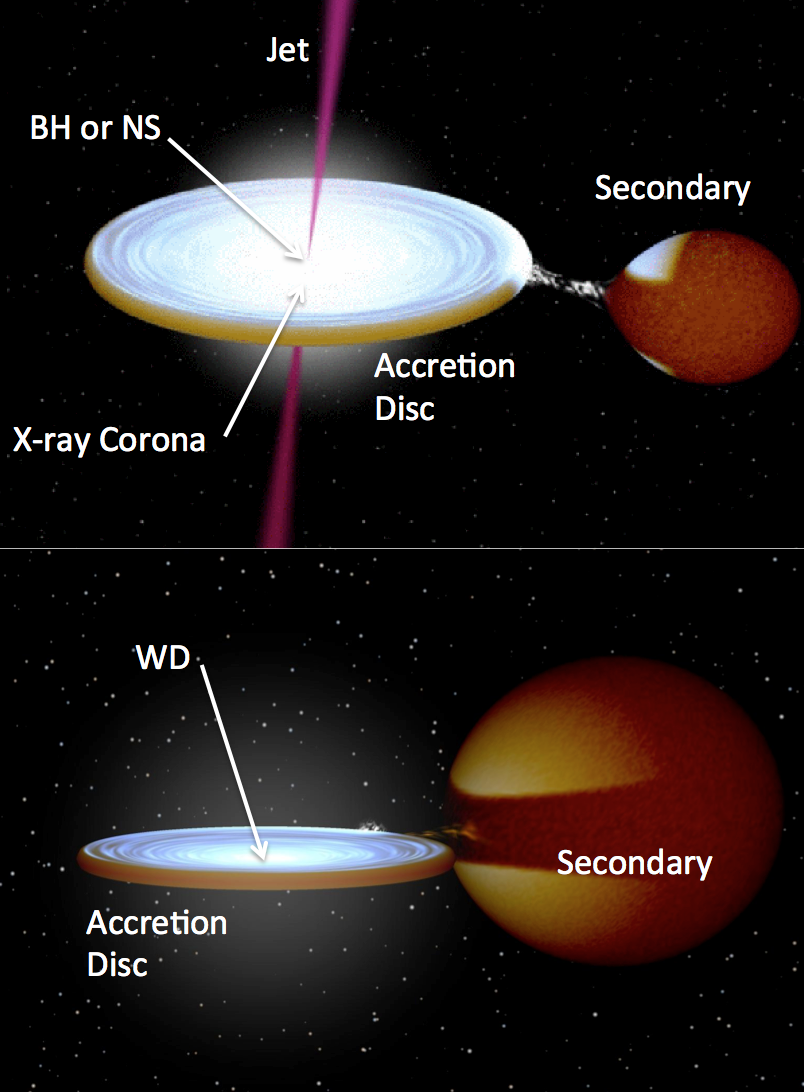
\includegraphics[width=1.0\textwidth]{figures/01-intro/cv_and_xrb.png}
\caption
[Artists impression of an LMXB and CV.]
{
{\sl Credit: Rob Hynes.} 
Artists impression of a low-mass X-ray binary (top) and
cataclysmic variable (bottom). The key components are marked,
and the clear similarity in overal structure is apparent.
} 
\label{fig:cv_and_xrb}
\end{figure}

Accreting compact binaries form many different classes, 
but are all characterised by matter streaming from a donor
onto a compact object. When the compact object is more massive 
than the donor then it is designated as the `primary', 
and the companion as the `secondary'. 
In high-mass X-ray binaries (HMXBs), the opposite is formally true.
There are only two ways by which matter can transfer 
from the secondary to the compact object. One is by Roche Lobe-overflow (RLOF),
whereby stellar evolution causes the donor star to fill its Roche Lobe, the surface
of equipotential around the star. The alternative is that the donor may expel
material via a disc or radiatively driven stellar wind, 
allowing some of it to flow onto the compact object. 
Although accretion from a wind or circumstellar disc is common in 
HMXBs \citep{bartlett2013}, here I will focus on 
RLOF as it is more common in the systems that possess high-state accretion discs
and associated outflows. Two examples of these are shown in figure~\ref{fig:cv_and_xrb}


\subsection{Roche Lobe-Overflow}

Let us consider a binary system, with masses $M_1$ and $M_2$, at positions
$\vec{r}_1$ and $\vec{r}_2$. The Roche potential, $\Phi_R$, in this system 
is then
\begin{equation}
\Phi_R = - \frac{GM_1}{| \vec{r} - \vec{r}_1 |} - 
\frac{GM_2}{| \vec{r} - \vec{r}_2 |} - 1/2 (\vec{\omega} \times
 \vec{r})^2,
\label{eq:roche}
\end{equation} 
where $\vec{\omega}$ is the angular velocity of the binary and is a vector normal to
the orbital plane. This potential is plotted in figure~\ref{fig:roche} for a mass ratio, 
$q = M_2 / M_1$ of 0.25.

\begin{figure}
\centering
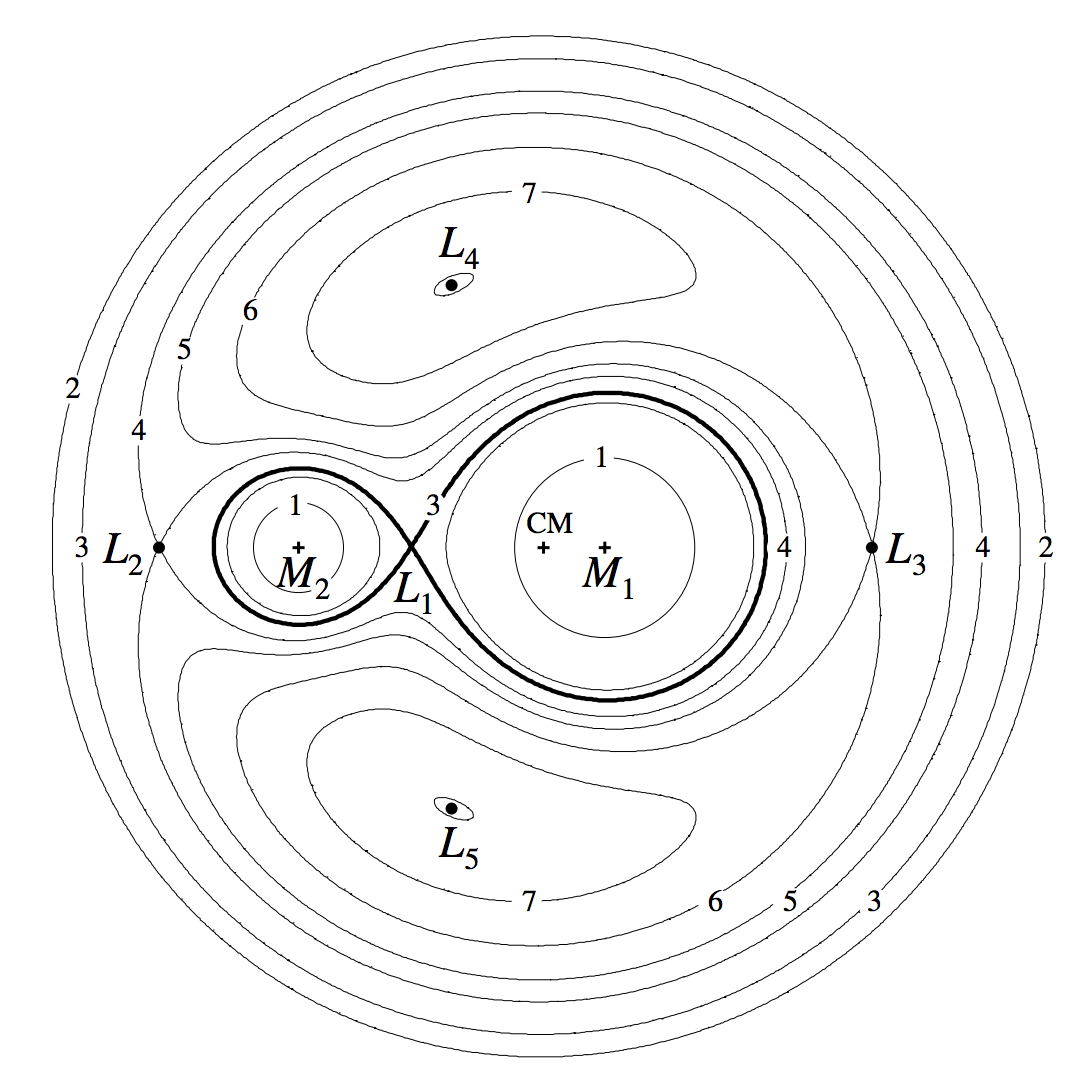
\includegraphics[width=0.7\textwidth]{figures/01-intro/roche_potential.png}
\caption
[The Roche potential in a binary system]
{
{\sl Credit: Frank et al. 2002.} 
The Roche potential in a binary system for $q = M_2 / M_1$ of 0.25.
The Lagrangian points are marked, as are the locations of the individual
and system centres of mass.
} 
\label{fig:roche}
\end{figure}

In the context of semi-detached binary systems, the most important region of the 
potential is the dumbbell shaped region enclosing the masses. Each of these
enclosed regions is known as the `Roche lobe' of the object and can be expressed 
approximately in terms of the mass ratio and separation of the system. A good approximation
for the size of the Roche lobe takes the form \citep{eggleton1983}
\begin{equation}
\frac{R_2}{a} = \frac{0.49 q^{2/3}}{0.6q^{2/3} + \ln(1+q^{1/3})}.
\label{eq:roche2}
\end{equation} 
Here $R_2$ is the radius of a sphere with the same volume as the Roche lobe for the
secondary star, which we can see depends only on $q$ and the orbital separation, 
$a$. If this secondary expands enough to fill its Roche lobe, then matter
will fall onto the other object. This process is known as Roche Lobe overflow (RLOF),
and is vitally important in astrophysics. Although caused by stellar evolution,
any accretion from RLOF will affect the mass ratio of the binary system 
and thus itself affects the evolution
of binary systems. This helps determine the orbital period
distribution of binaries \citep[e.g.][]{knigge2011_evo} 
as well as affecting the delay time distribution
of Type Ia Supernovae, for which CVs are one of the progenitor candidates 
\citep[e.g.][]{wang2012}.
It is also worth noting that the existence of gravitational waves has been 
required in models to explain the orbital period evolution of CVs since
the 1960s \citep{kraft1962}. 


\subsection{Cataclysmic Variables}

Cataclysmic variables (CVs) are systems in which a WD
accretes matter from a donor star via Roche-lobe overflow 
\citep[see the `CV bible', ][]{warnerbook}. 
CVs are not always dominated by their accretion luminosity; 
classical novae and super soft sources 
(SSS) emit mostly due to nuclear burning or detonation on the WD surface.
Accretion dominated CVs -- the focus here -- can be classified according to the 
magnetic field strength of the WD ($B_{WD} $) and photometric activity. 
Magnetic systems are classified as either `Polars' ($B_{WD} \gtrsim 10^7$~G)
or `Intermediate Polars' ($10^6 \lesssim B_{WD}  \gtrsim 10^7$~G);
in these systems the accretion flow inside the some critical radius 
(related to the Alfven radius)
is dominated by the WDs magnetic field \citep[e.g.][]{patterson1994}. 
In polars, this radius is large enough, due to the strong magnetic field,
that no disc forms at all \citep{liebert1985}.
When $B_{WD}  \lesssim 10^6$~G then the accreting material can fall
onto the WD via a disc, and the CV is classified as non-magnetic.
There are two main types of non-magnetic CVs; dwarf novae and nova-like
variables.

\subsubsection{Dwarf Novae and the Disc-instability Model}

Dwarf novae (DNe) are CVs that are characterised 
by repeated periods of quiescence and dramatic outburst. One of the 
most famous DNe is SS Cyg, whose light curve is shown in 
figure~\ref{fig:sscyg}. The repeated outbursts can be clearly seen, and
SS Cyg itself has been undergoing this behaviour for the full century 
for which it has been observed. A spectrum over the course of a 
typical outburst is shown in figure~\ref{fig:sscyg_spec}, 
and is characterised by the appearance of an optically thick
accretion disc continuum -- note the similarity to the 
stellar atmosphere disc spectrum computed in section~\ref{sec:alpha_disc},
and to the intermediate inclination nova-like variables discussed in the next
section.

The leading scnario for explaining DN outbursts, and in fact also the outbursts
in low mass X-ray binaries or `soft X-ray transients',
is the disc-instability model 
\citep[DIM; ][]{osaki1974,lasota2001}. 
In this model, a gradual increase in supply rate from the donor star 
(and hence surface density in the disc) 
causes the disc to heat up. Eventually, the disc hits a critical temperature,
around $7000$~K, and becomes ionized. Now the surface density in the disc
can increase significantly, and the disc becomes geometrically thin and
optically thick. Most importantly, it can undergo efficient radiative
cooling, and a significant increase in brightness is observed.

\begin{figure}
\centering
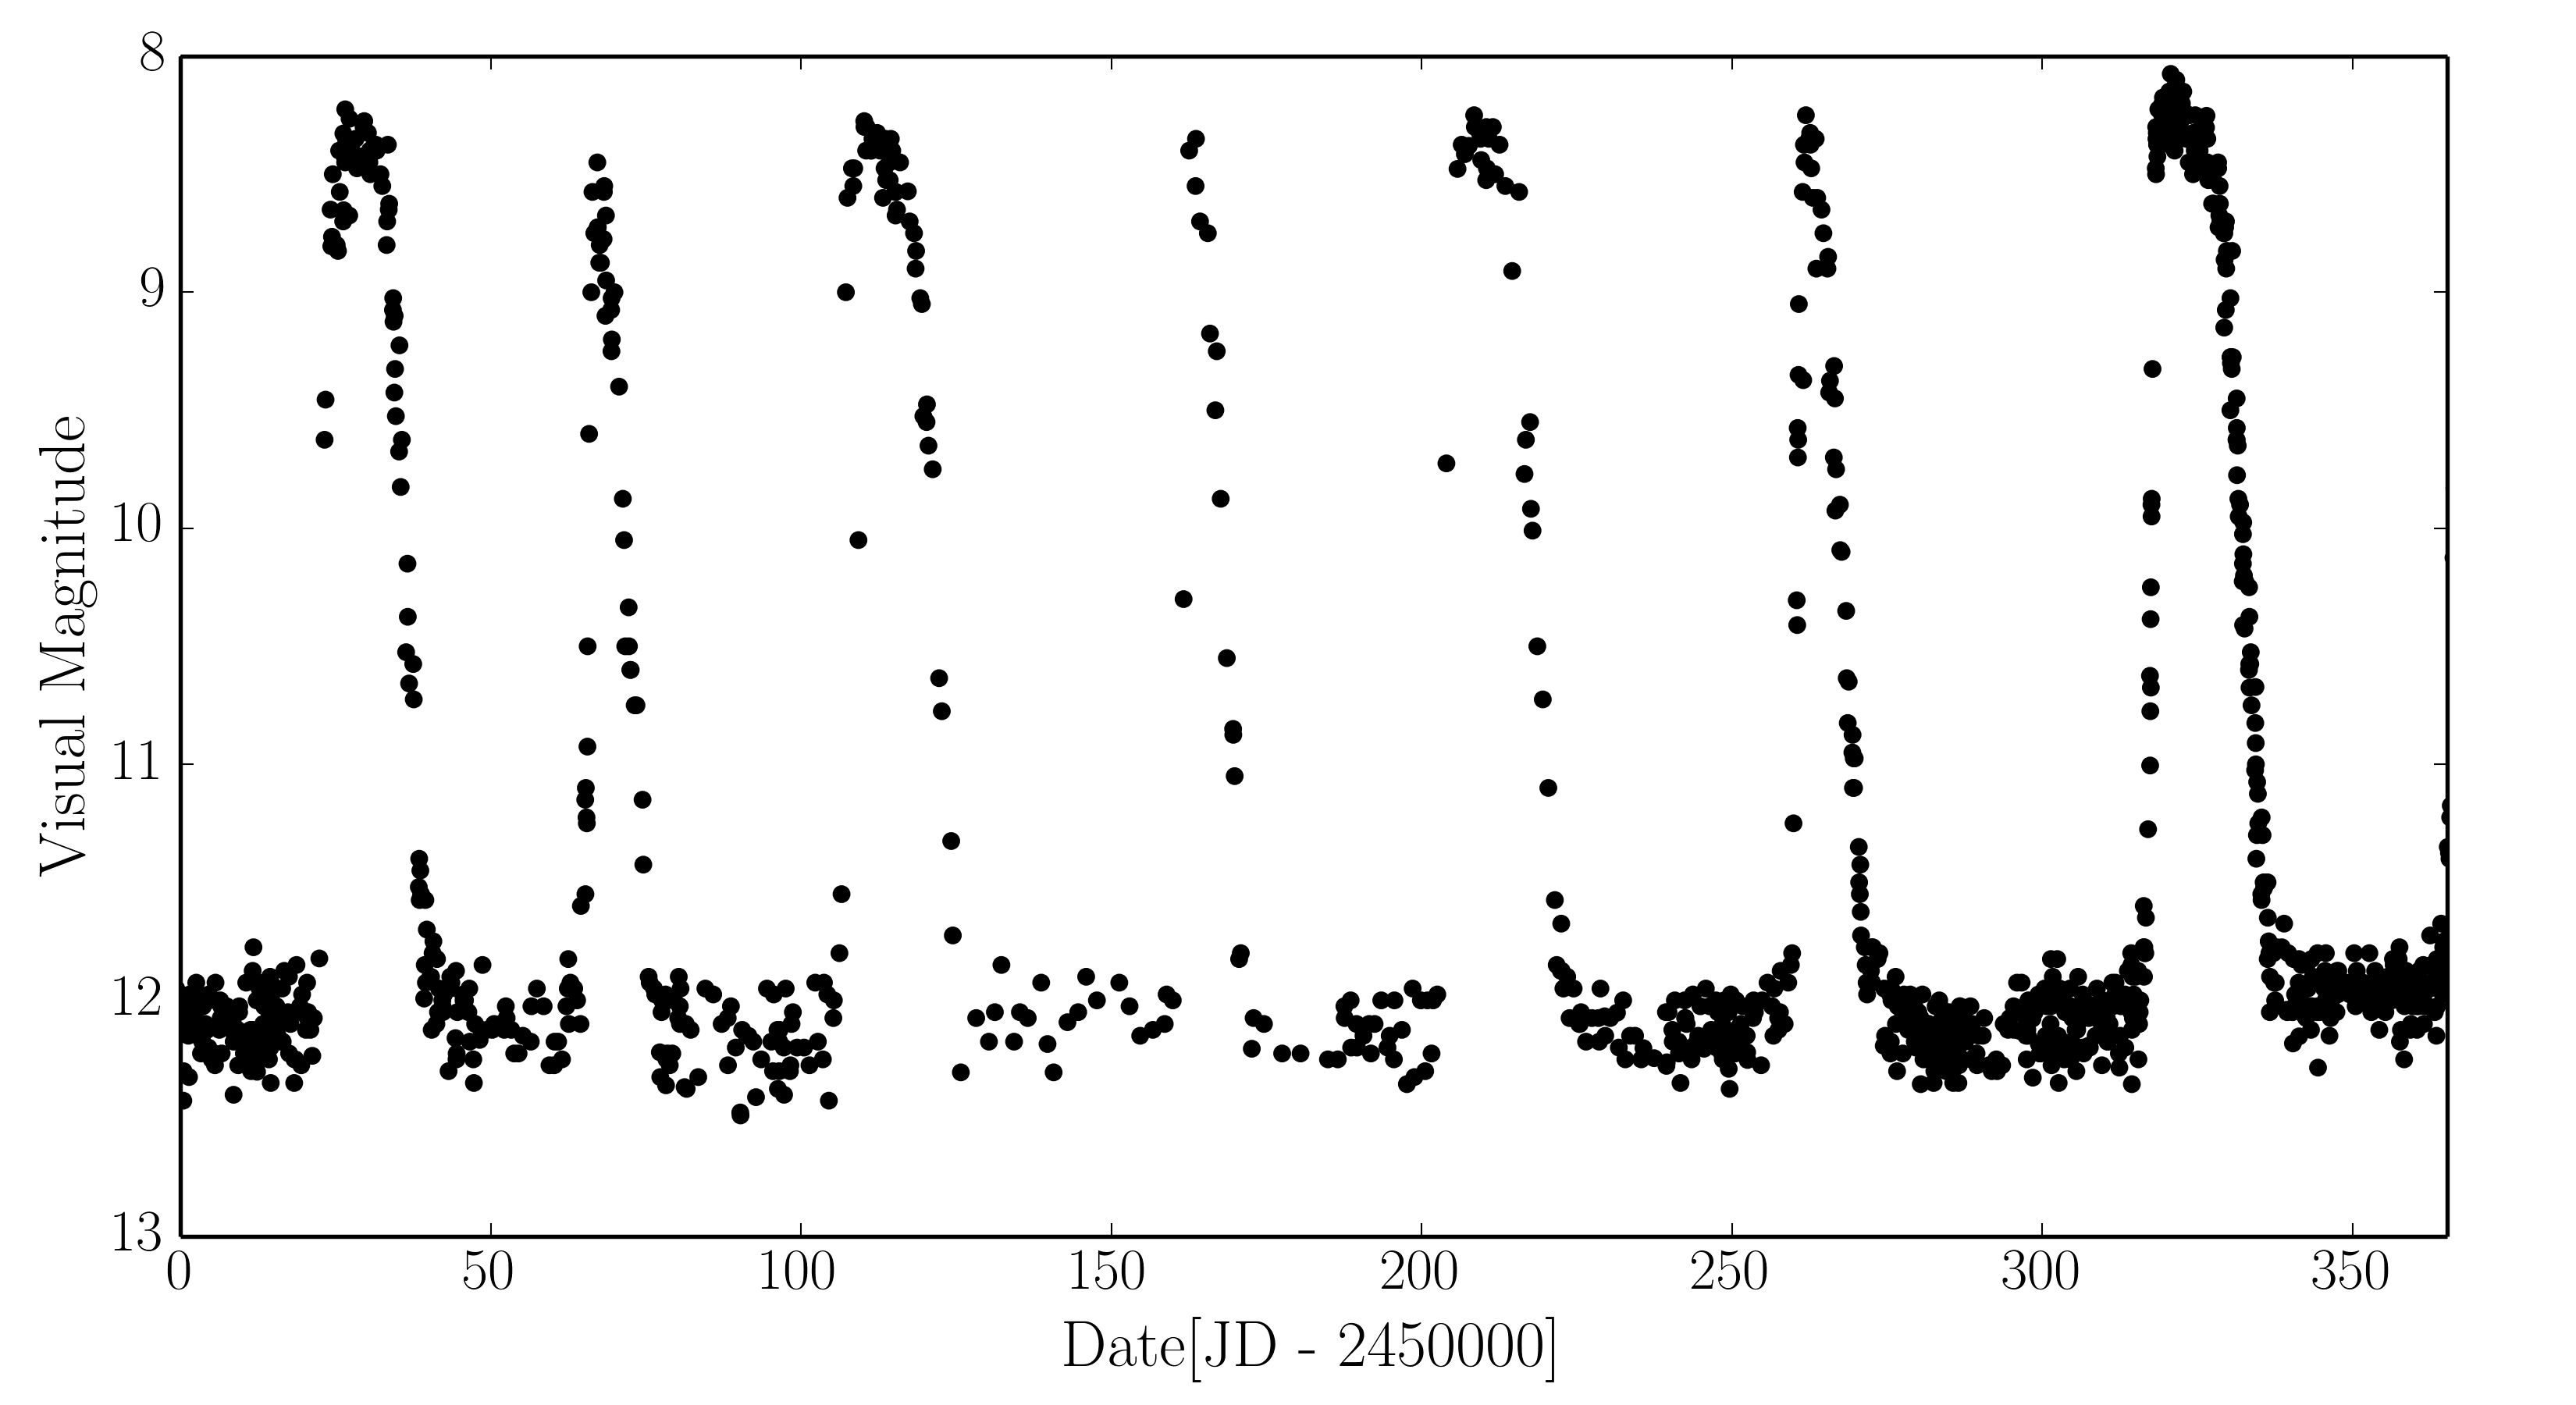
\includegraphics[width=1.0\textwidth]{figures/01-intro/lc_sscyg.png}
\caption
[A year in the life of SS Cyg.]
{
{\sl Data: AAVSO.} 
A year in the life of SS Cyg, showing the characteristic repeated
outbursts and periods of quiescence typical of a DN. SS Cyg has been
undergoing this activity since it was first observed in 1896.
} 
\label{fig:sscyg}
\end{figure}

\nocite{dhillon1996,hessman1984}
\begin{figure}
\centering
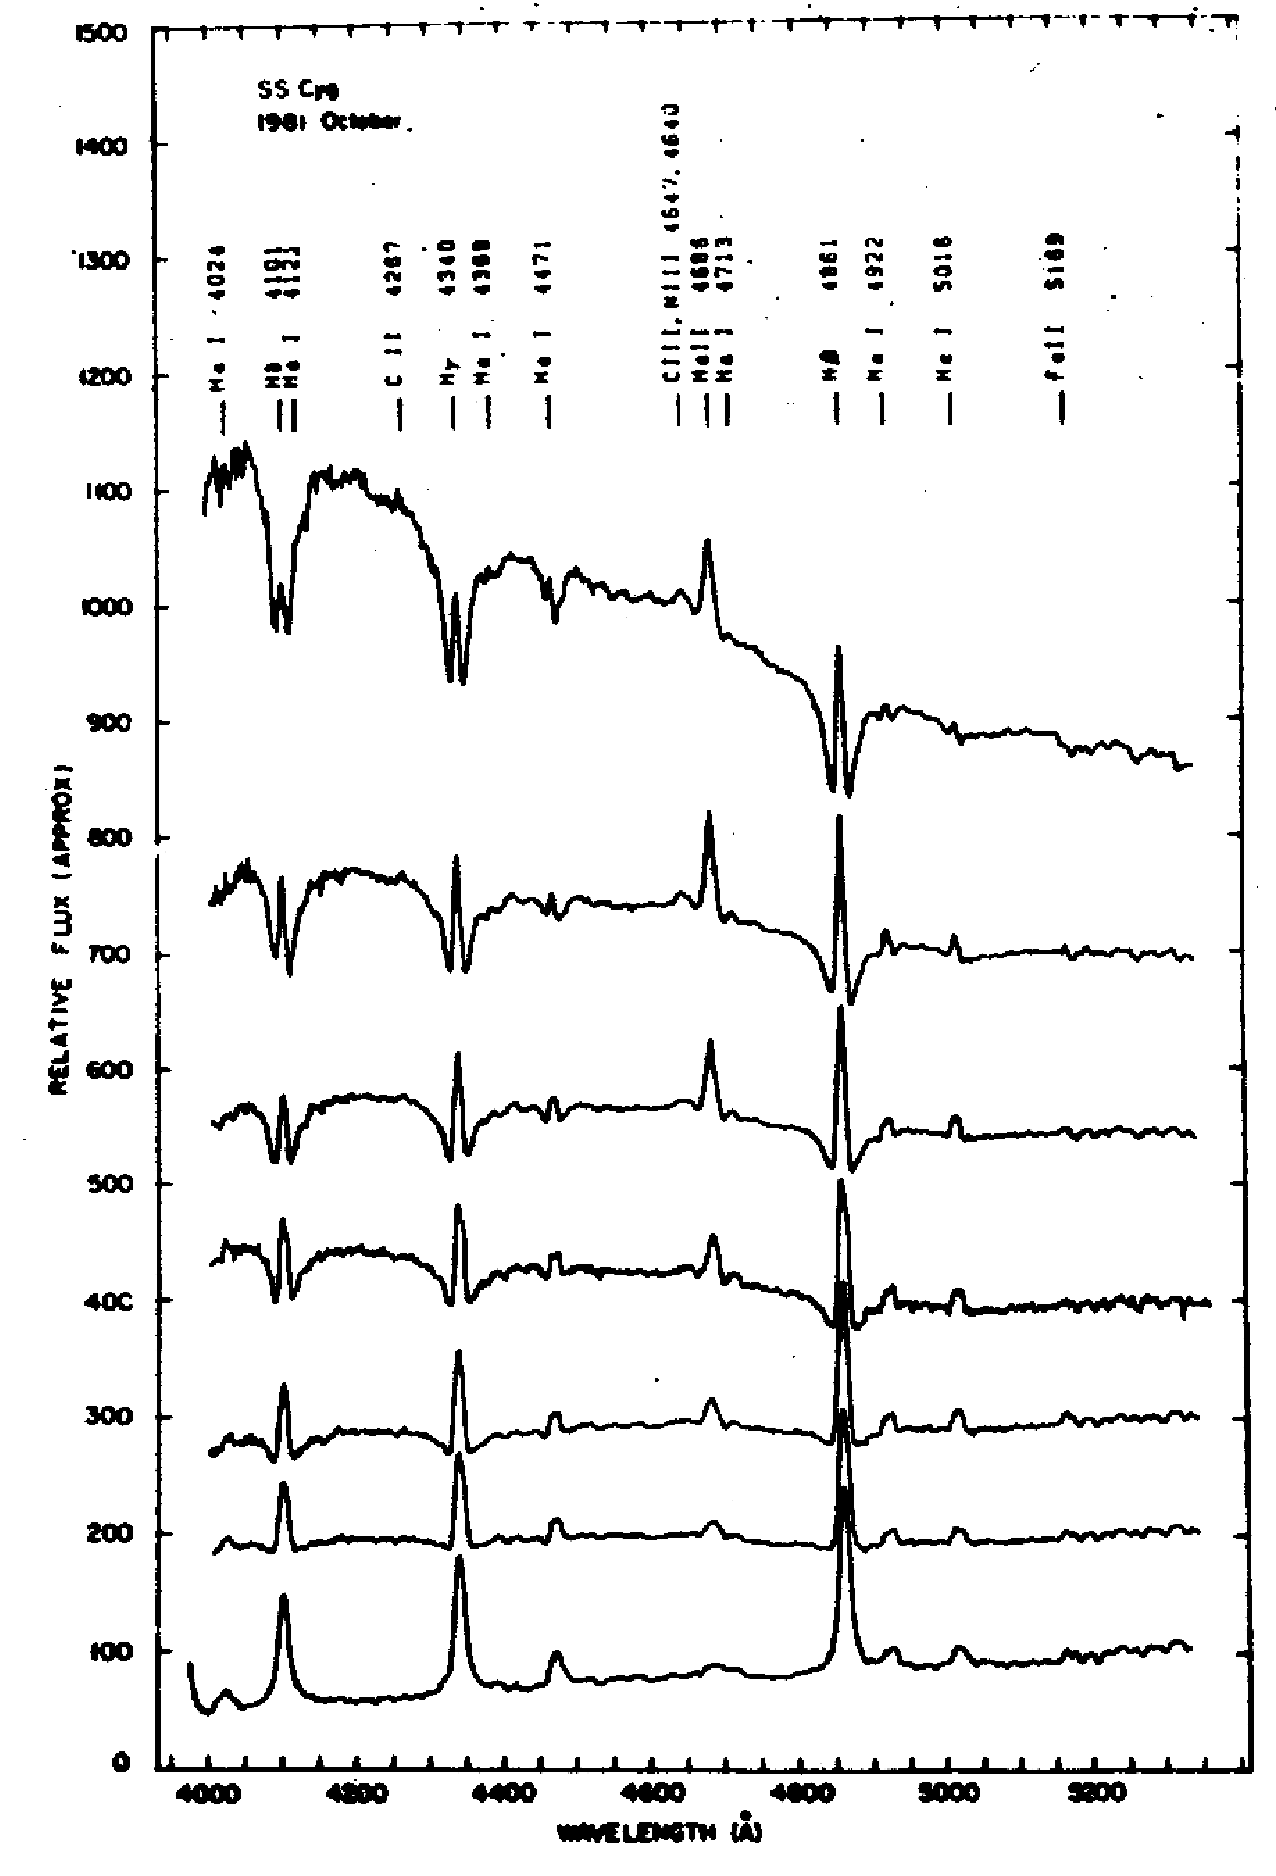
\includegraphics[width=1.0\textwidth]{figures/01-intro/sscyg_spec.png}
\caption
[Spectra of SS Cyg during an outburst cycle]
{
{\sl Credit: Hessman et al. 1984 / Dhillon et al. 1996.} 
Spectra of SS Cyg during an outburst cycle, showing the evolution from 
minimum to maximum light. The rise is characterised by the appearance of an
optically thick accretion disc spectrum. The flux scale is approximate.
} 
\label{fig:sscyg_spec}
\end{figure}

\subsubsection{Nova-like Variables}

\nocite{dhillon1996,hessman1984}
\begin{figure}
\centering
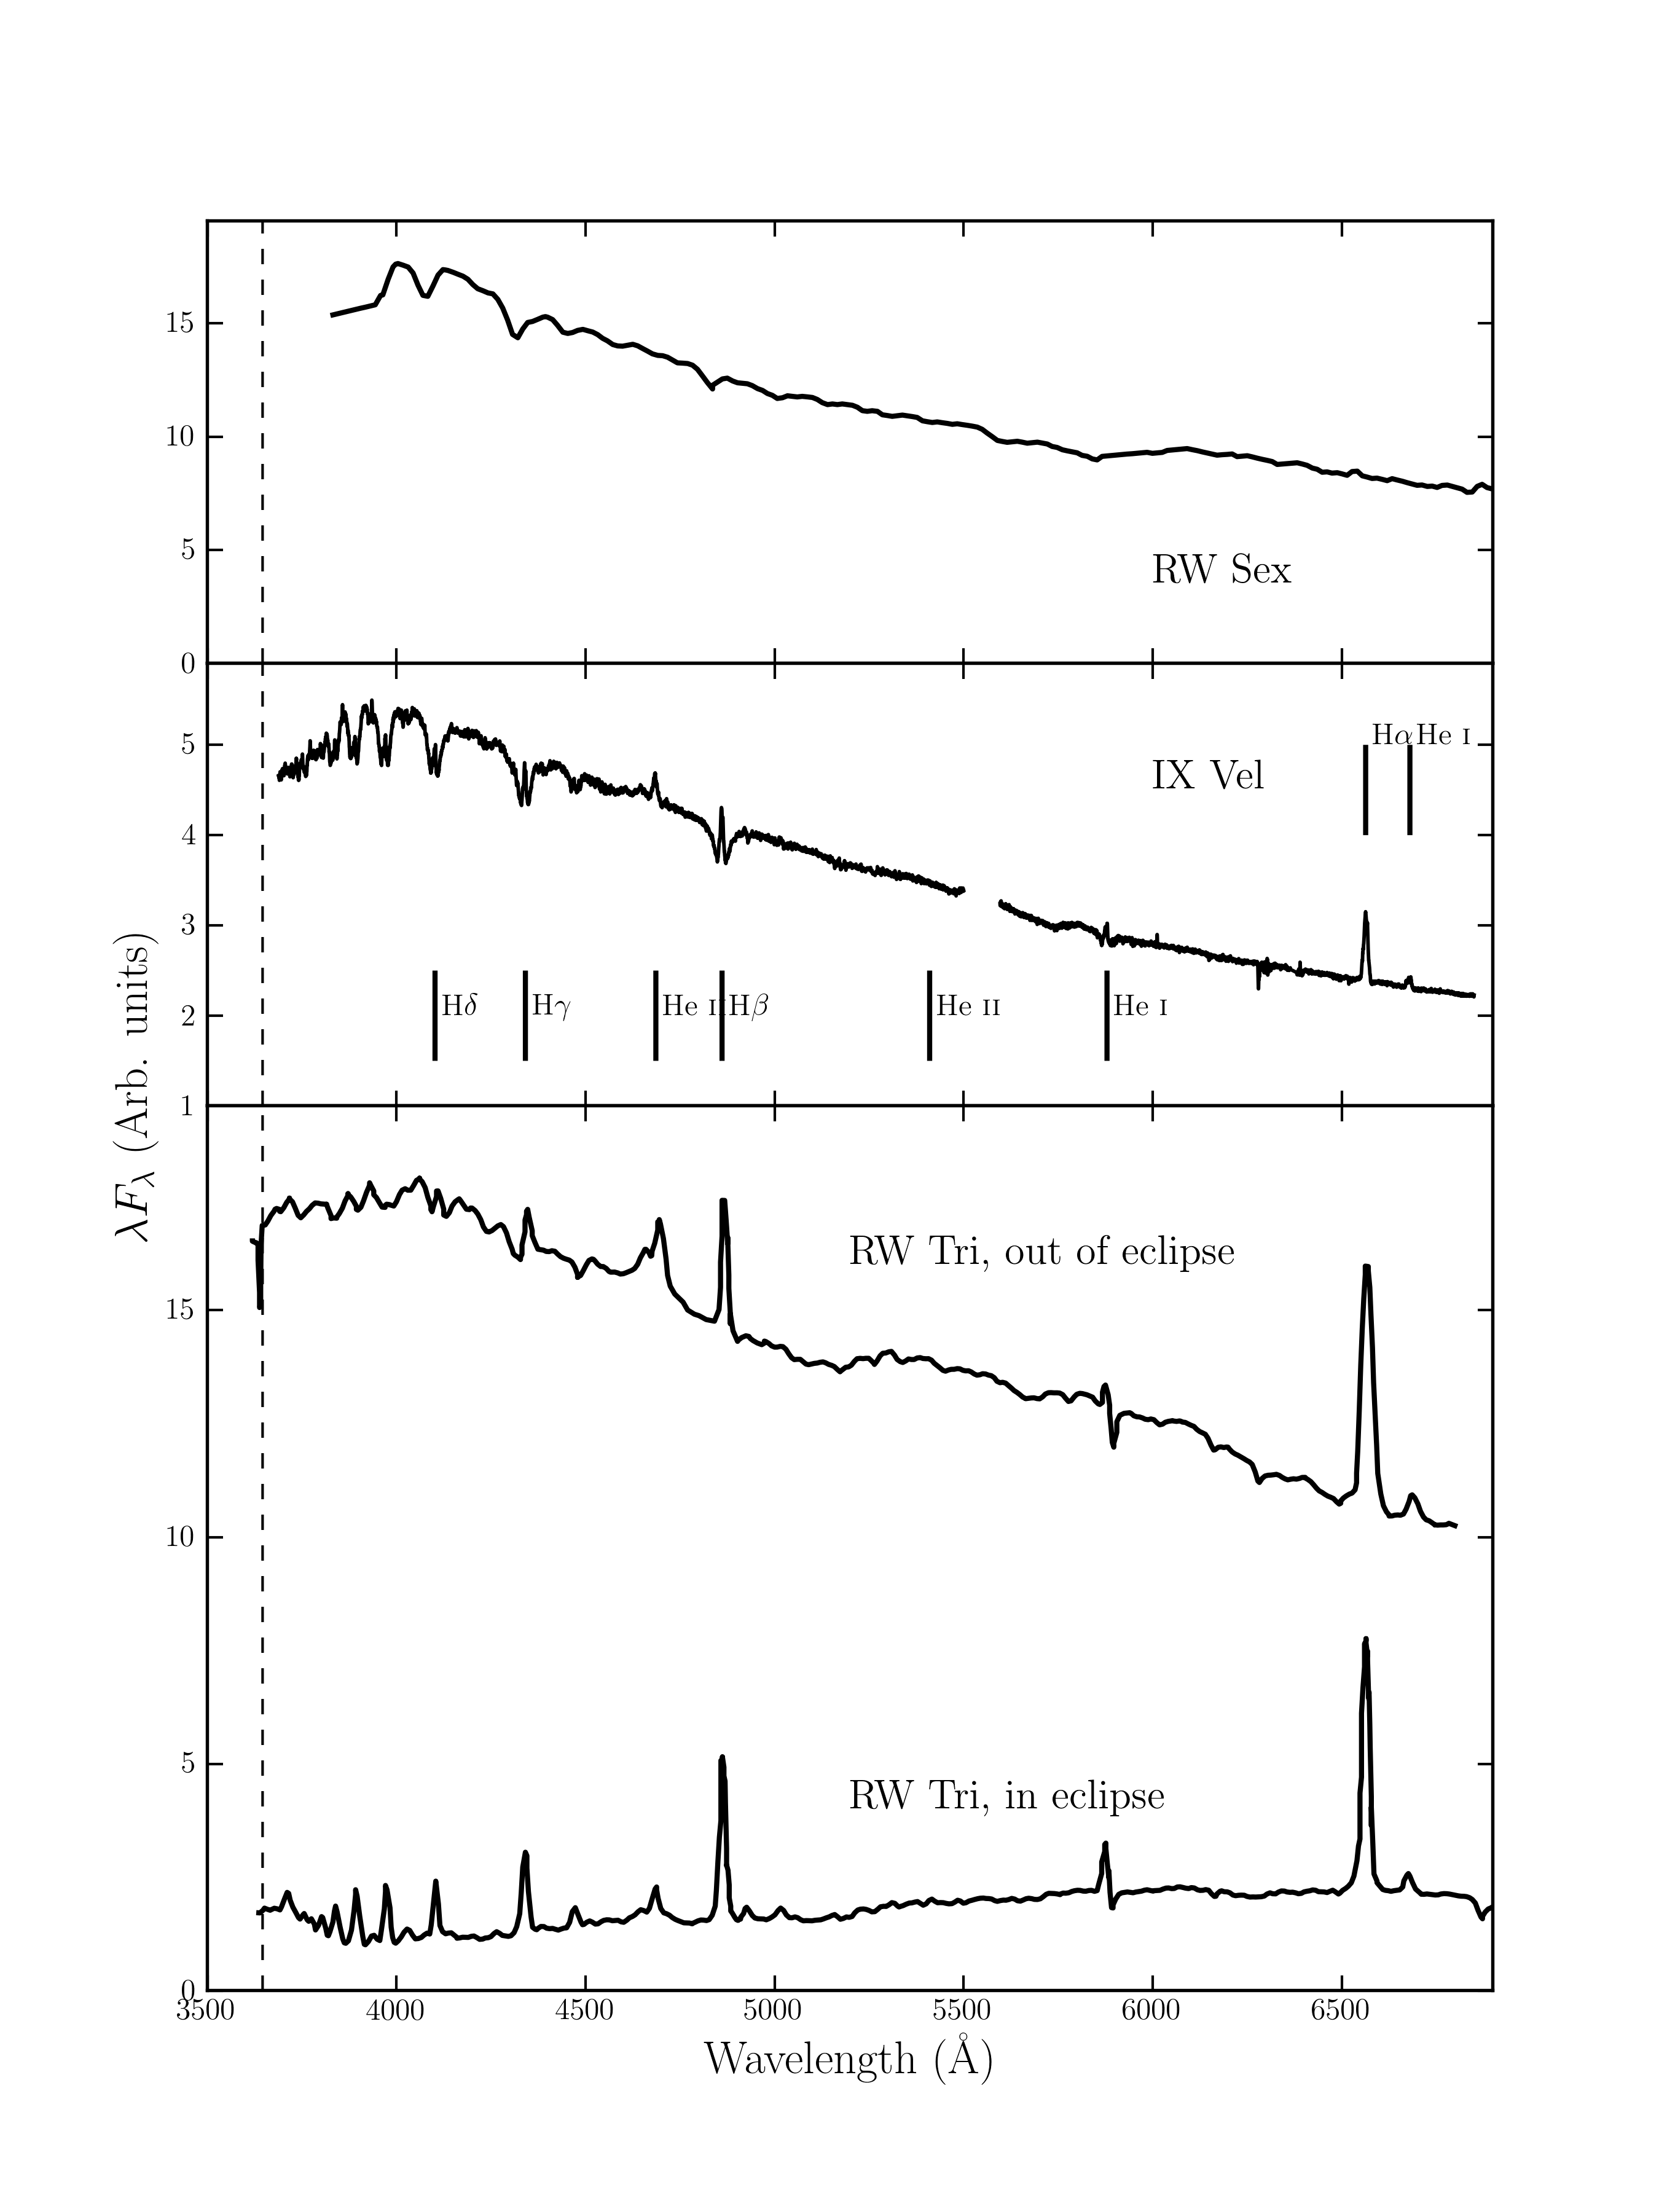
\includegraphics[width=1.0\textwidth, clip=true, trim= 0 0.6in 0 0.8in]{figures/01-intro/novalikes.png}
\caption
[Optical spectra of three nova-like variables.]
{
Optical spectra of three nova-like variables: 
RW Sex (top; Beuermann et al. 1992),
IX Vel (top middle; A. F. Pala \& B. T. Gaensicke, private communication) 
and RW Tri in and out of eclipse (bottom two panels; Groot et al. 2004).
The data for RW Sex and RW Tri were digitized from the respective publications,
and the IX Vel spectrum was obtained using the XSHOOTER spectrograph 
on the Very Large Telescope on 2014 October 10.
These systems have approximate inclinations of 
$30^\circ$, $60^\circ$ and $80^\circ$ respectively. 
The trend of increasing Balmer line emission with inclination can be seen.
In RW Tri strong single-peaked emission in the Balmer lines is seen even
in eclipse, indicating that the lines may be formed in a spatially
extensive disc wind, and there is even a suggestion 
of a (potentially wind-formed) recombination continuum in the eclipsed
spectrum. I have attempted to show each spectrum over a similar dynamic range.
} 
\label{fig:NL_spec}
\end{figure}

Nova-like variables (NLs) are similar to DNe,
except that the disc is always in a relatively 
high-accretion-rate state ($\dot{M} \sim 10^{-8}$~M$_{\odot}$~yr$^{-1}$).
NLs are therefore one of the best `laboratories' for testing the steady-state
accretion disc theory described in section~\ref{sec:alpha_disc}.
In the optical, NLs generally exhibit a series of H and He emission 
lines superposed on a blue continuum. In many
cases, and particularly in the SW~Sex subclass of NLs
\citep{HSK86,DR95}, these lines are single-peaked. This is contrary to
theoretical expectations for lines formed in accretion discs, which
are predicted to be double-peaked \citep{smak1981, hornemarsh1986}. 
{\em Low-state} CVs (dwarf novae in quiescence) do, in fact,
exhibit such double-peaked lines \citep{marshhorne1990}. 

\nocite{dhillon1996,hessman1984}
\begin{figure}
\centering
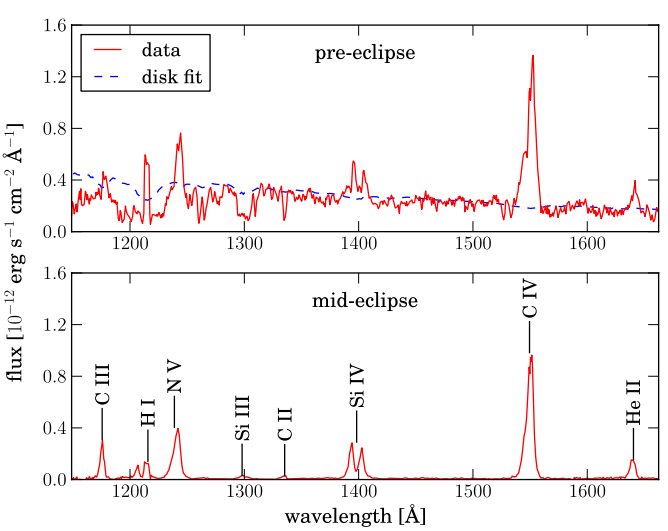
\includegraphics[width=1.0\textwidth]{figures/02-outflows/rwtri_noe.png}
\caption
[UV spectrum of RW Tri in and out of eclipse.]
{
{\sl Credit: Noebauer et al. 2010}.
UV spectrum of RW Tri in and out of eclipse, showing strong lines in 
\civfull\ and \la, among others.
} 
\label{fig:NL_spec}
\end{figure}


The UV spectra of NLs also show strong emission lines, and at 
low to intermediate inclinations dramatic blue-shifted absorption lines
can be seen in some objects. The emission line equivalent widths
in both the optical and the UV show clear correlations with 
inclination \citep{hessman1984,echevarria1988,noebauer}. 
This can be seen clearly in figure~\ref{fig:NL_spec}, and is connected to
the correlation between line strength and absolute magnitude found by \cite{patterson1984};
that is, the decrease in equivalent width at low inclination is caused by an {\em increase}
in continuum flux. This is discussed further in chapters 4 and 6, but also has 
relevance to AGN and quasar unification schemes mentioned later in this introduction.
The optical and UV spectra of NL CVs are discussed further
in the context of winds in chapter 2.

\subsection{Low Mass X-ray Binaries}

Low-mass X-ray binaries (LMXBs) 
are similar to CVs in structure (see figure~\ref{fig:cv_and_xrb}), 
but the compact object
is either a neutron star (NS) or black hole (BH). The accretion disc 
emits in the soft X-ray regime, and an additional hard X-ray power law is also 
seen in the spectrum. This hard component is normally attributed
to Compton up-scattering of seed disc photons by some kind of `corona'
of hot electrons close to the BH \citep[e.g.][]{white1988,mitsuda1989,uttley2014}.
Although I do not study LMXBs directly in this thesis, it is instructive
to briefly discuss of their observational appearance as it is relevant to the links
between accretion and outflow. The discovery that XRBs and CVs follow similar 
tracks on a hardness-intensity diagram \citep[HID;][]{kordingDNjet2008}
is particularly interesting in this regard, especially since \cite{ponti2012}
showed that broad Fe absorption lines are only seen in the soft-state 
high-inclination systems (see section~\ref{sec:xrb_winds}). 
This implies that equatorial outflows are intrinsic to 
the accretion process. Although the driving mechanism
is probably different to CVs \citep[e.g.][]{diaztrigo2015}, 
the similarity in general structure to models for CVs and quasars is striking.


% \begin{figure}
% \centering
% 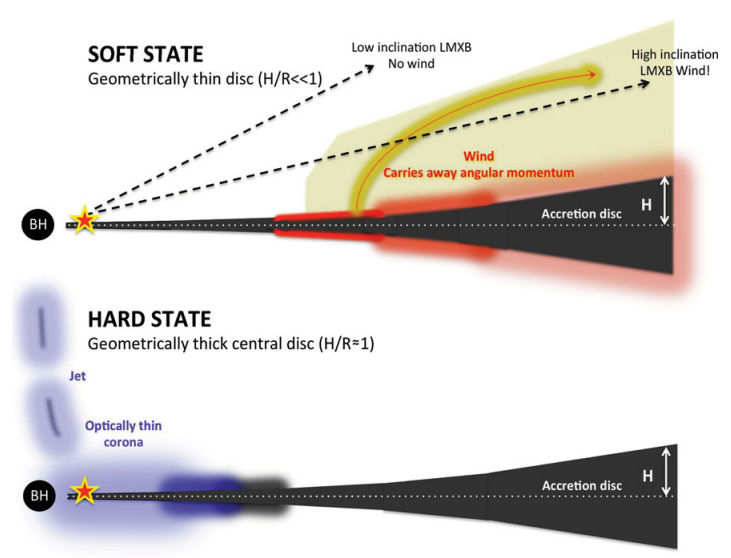
\includegraphics[width=0.7\textwidth]{figures/01-intro/ponti_wind_cartoon.png}
% \caption
% [Hardness intensity diagram for a WD, NS and BH system]
% {
% {\sl Credit: Ponti et al. 2012}
% Hardness intensity diagram for a WD, NS and BH system
% } 
% \label{fig:ponti_cartoon}
% \end{figure}


\section{Quasars and Active Galactic Nuclei}

Spectra of AGN have now been studied for over 100 years, and we have known 
that they exhibit strong, broad emission lines since the first spectrum was taken by
\cite{fath1909}. However, it wasn't until the work of \cite{seyfert1943} that the systematic 
classification of AGN really began, leading to the phrase `Seyfert galaxy'.
This label was applied to galaxies possessing a bright nucleus, spectroscopically
characterised by a blue continuum and a series of strong emission lines.
The first real physical insight into the extraordinary nature of AGN
was provided by \cite{woltjer1959}, who noted that 
(i) the nuclei must have sizes $<100$~pc,
based on the fact that they were unresolved, and (ii) the mass of the nucleus
must be very high, based on virial estimates. 
While both of these observations were based on simple arguments, the fact that these
ultra-luminous celestial objects are both {\em compact} and {\em supermassive}
is perhaps the defining insight into the nature of AGN.

Although the study of AGN was established in the optical waveband, 
radio astronomy also significantly furthered our understanding of AGN
in the mid-20th century. A number of surveys, such as the Cambridge \citep{edge1959}, 
Parkes \citep{ekers1969} and Ohio \citep{ehman1970} surveys discovered a great many 
bright radio point sources distributed isotropically across the sky.
These sources eventually became known as `quasi-stellar radio sources',
or {\em quasars}, and were soon found to be coincident with bright optical
sources or `quasi-stellar objects' (QSOs) at high 
redshifts \citep{schmidt1963,schmidt1965a,schmidt1965b}.
Nowadays, the term quasar normally has very little to do with 
radio emission and is often used interchangeably with QSO. 
Indeed, throughout this thesis I shall refer to a quasar as simply a bright, 
massive AGN; one with sufficiently high luminosity that it dominates the emission 
from its host galaxy.

One of the main classification schemes for AGN is a spectroscopic one, based on 
whether an object possesses broad emission lines in its spectrum, 
such as \civ\, broad \hb\ and
\la, in addition to the narrow lines that are always present. 
If these broad lines are seen, then the AGN is classed as type I;
if not, it is classed as type II (figure~\ref{fig:agn_templates}).
These designations were originally applied to Seyfert galaxies \citep{seyfert1943}, 
but can also be used to classify the more luminous quasar class, despite the apparent
difficulty in finding the expected number of type II sources \citep{zakamska2003}. 
This classification scheme is complicated somewhat by the existence of two
unusual types of AGN: narrow line Seyfert Is (NLSIs), which
may be explained by super-Eddington accretion \citep{done2015} 
or perhaps simply an orientation effect \citep{baldi2016},
and so-called `true type II' AGN, in which the broad line region is absent 
\citep{tran2001,shi2010} rather than obscured (see next section).
Despite this muddying of the waters, what was originally a 
clear dichotomy in spectral type provided a 
profound motivation for attempting to {\em unify} AGN via geometric arguments.


% \subsection{AGN Taxonomy}
% \label{sec:agn_taxonomy}

% In addition to Seyfert galaxies and quasars, there are a number of 
% different classes of AGN. These are broadly characterised by their spectra in the 
% optical, UV and X-ray as well as their radio behaviour. It is worth noting
% that these are observational classifications; that is, even after a century
% of study, the {\em physical} origins of the diverse behaviour of AGN
% are still an active area of research.

\begin{figure}
\centering
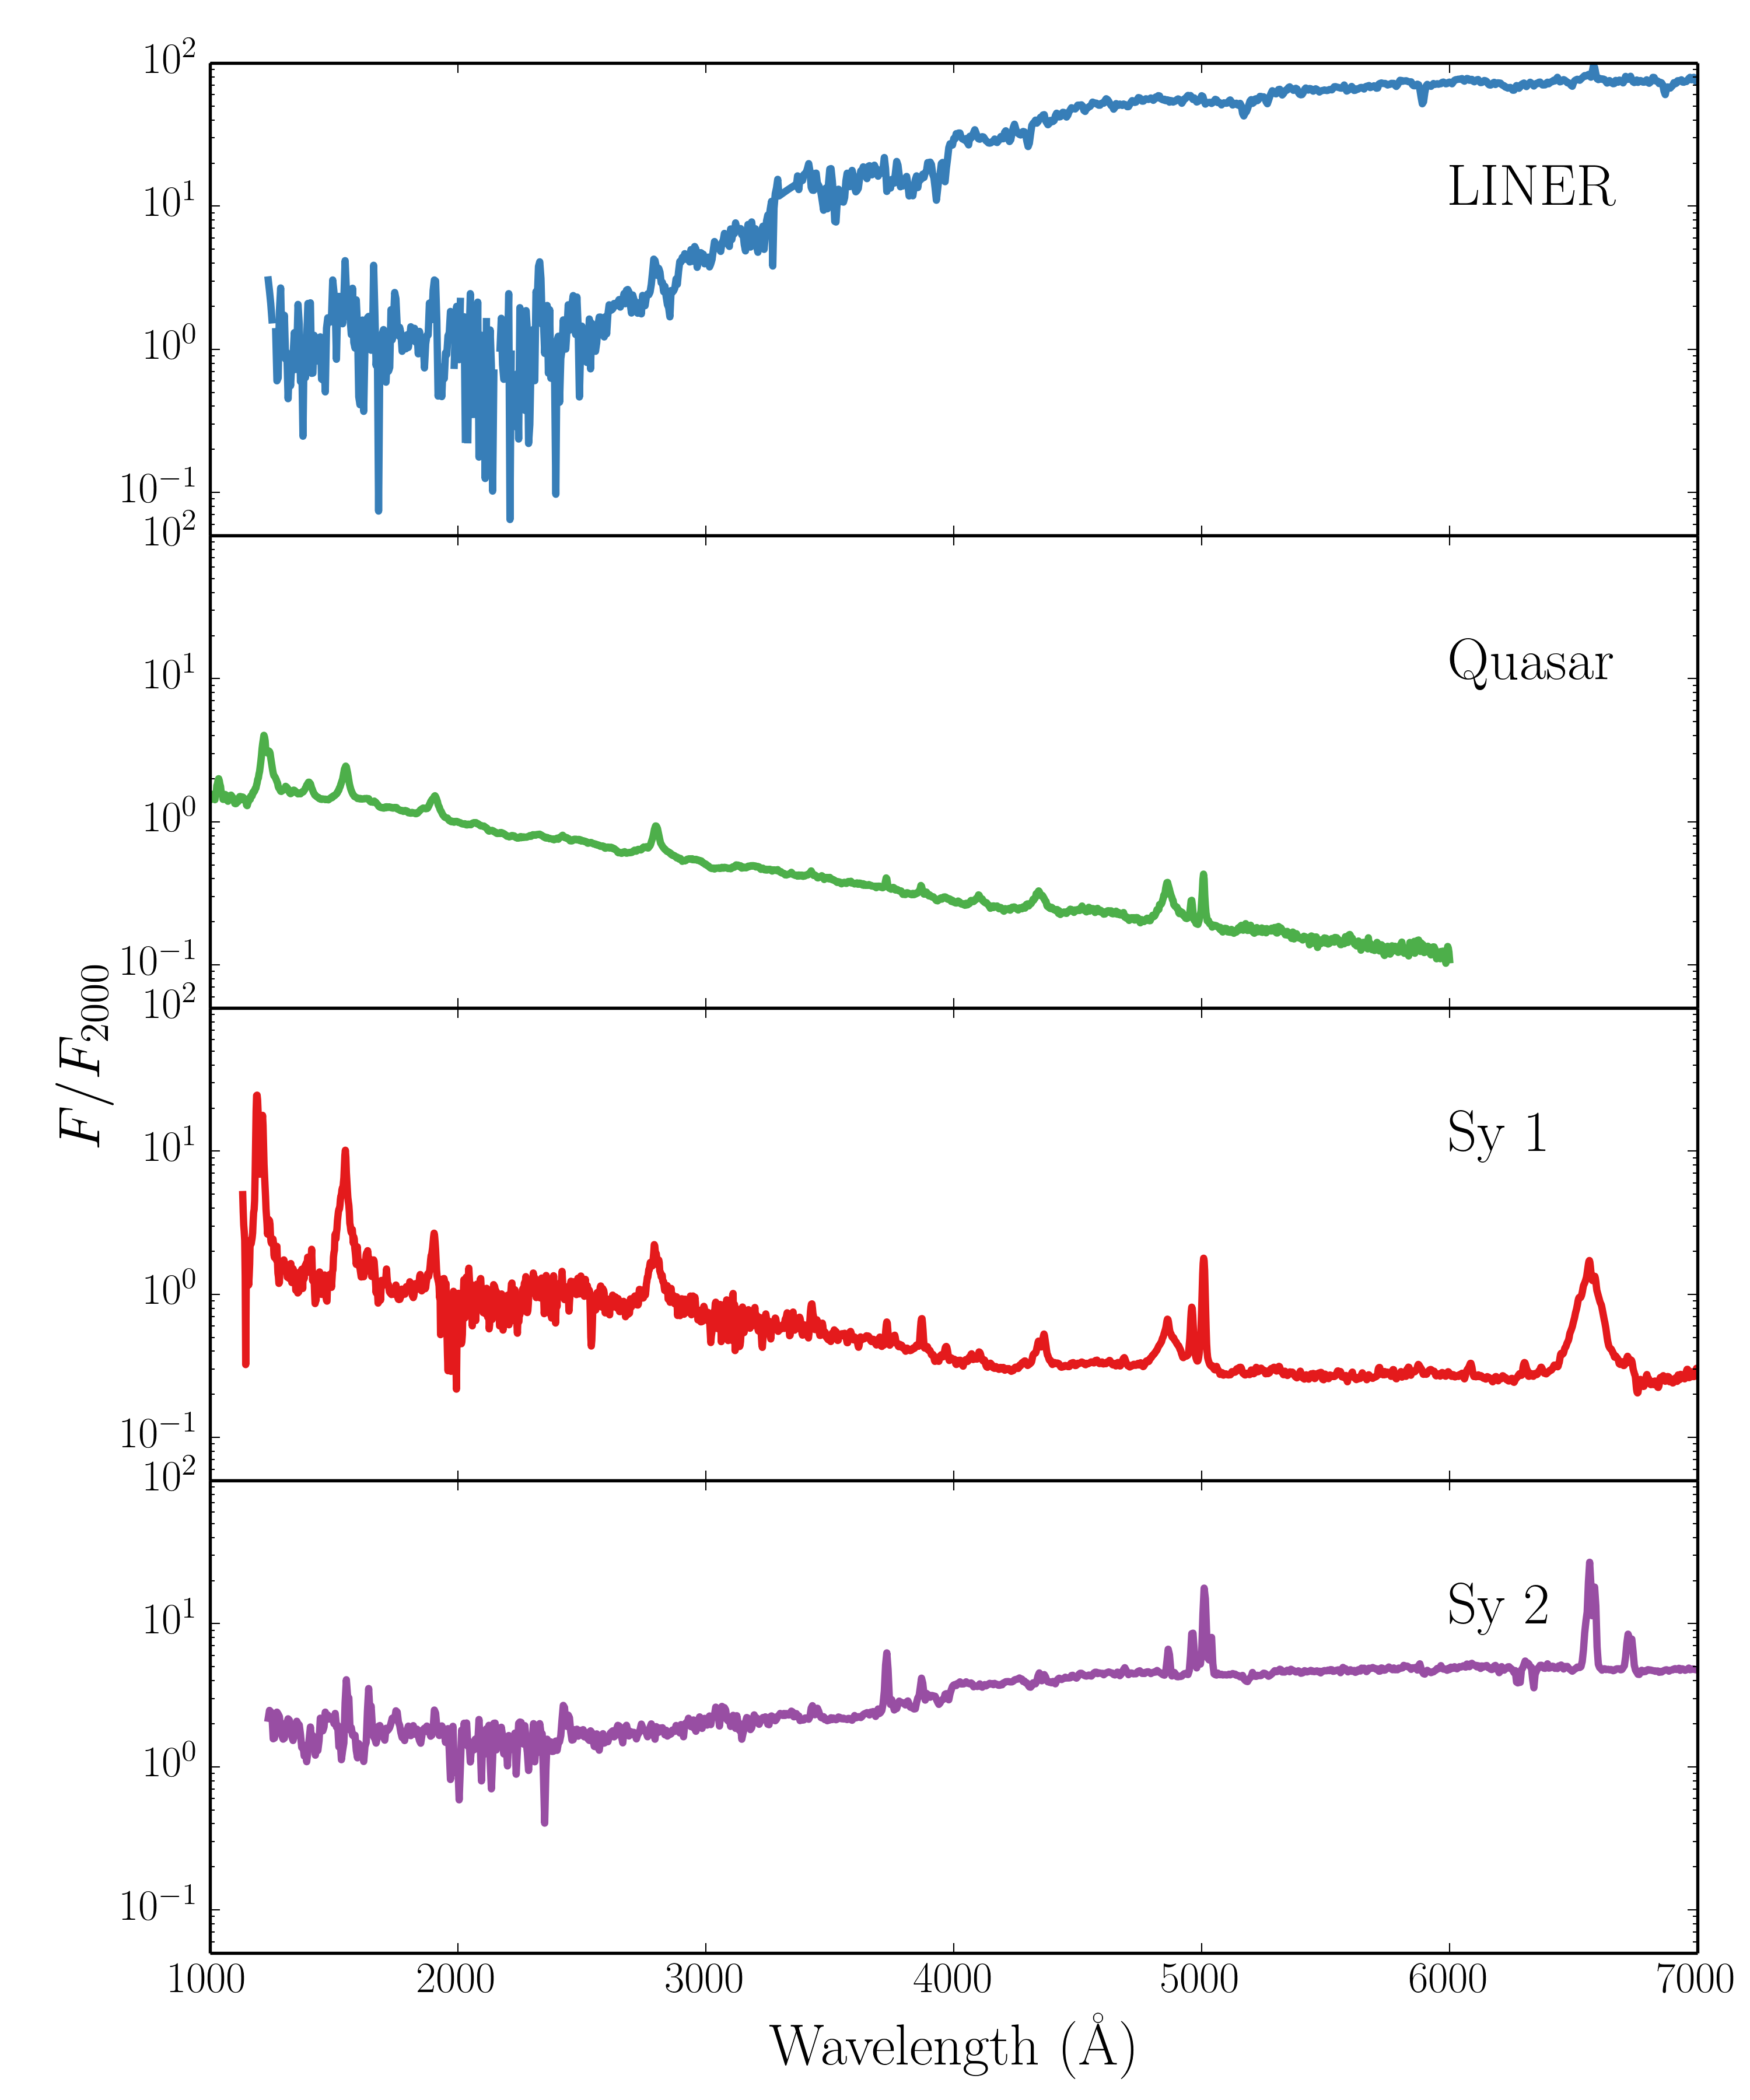
\includegraphics[width=1.0\textwidth]{figures/01-intro/agn_templates.png}
\caption
[Template spectra, from the AGN atlas, for four common types of AGN.]
{
Template spectra, from the AGN atlas, for four common types of AGN.
Obtained from \url{http://www.stsci.edu/hst/observatory/crds/cdbs_agn.html}.
} 
\label{fig:agn_templates}
\end{figure} 

% \subsubsection{Radio Galaxies}

% Radio galaxies are a broad class of AGN, of which radio-loud quasars and blazars are
% technically members, which show strong emission in the radio band. 
% The main classification scheme was proposed by \cite{FR1974}, who split
% sources according to the luminosity. FR I sources are lower in radio luminosity with a steadily decreasing surface brightness towards the edge of the radio lobes.
% FR II sources are more luminous and exhibit bright structures at the edge of their 
% radio maps. Radio galaxies are not particularly relevant here, but it is worth 
% noting that `Radio core dominance', $\log R$, is often used as an orientation indicator 
% \citep{orr1982,wills1995}. This is because more pole-on sources should, in theory, 
% be more dominated by their
% cores whereas edge-on sources should be more dominated by extended radio
% lobes. I discuss the use of orientation indicators further in chapter 6.

% \subsubsection{BL Lacs and Blazars}

% BL Lac objects -- named for the first object of the class, BL Lacertae --
% are AGN with featureless non-thermal continua 
% \citep[see figure~\ref{fig:agn_templates}, and][for a review]{falomo2014},
% in contrast to Seyfert galaxies. 
% Their optical flux is highly polarised \citep{angelstockman1980}
% and they tend to exhibit large-scale optical variability, 
% to the extent that they were originally classified as irregularly variable
% stars \citep{hoff1929}. BL Lacs are a subset of 
% a larger AGN class known as Blazars, the most luminous of which
% are known as optically violent variable (OVV) quasars \citep{wright1998}. 
% Blazars require relativistic beaming in order to explain their high 
% radio luminosities \citep{ghis1985,ghis1993}, 
% implying that the jet is orientated towards
% the observer. These objects thus have an important place in unification
% schemes (see section~\ref{agn_unification}), and
% allow us to measure bulk Lorentz factors in radio jets, which
% can be as high as $\sim50$ \citep{begelman2008}.

% \subsubsection{Obscured and Compton-thick AGN}

% \subsubsection{Low-luminosity AGN}


\subsection{AGN Unification and the dusty Torus}
\label{agn_unification}

Although Seyfert had identified type 1 and 2 AGN, a physical explanation
for this dichotomy was not forthcoming until a study by \citet[][AM85]{antonucci1985}.
They showed unambiguously that the nearby Seyfert 2 NGC~1068 is simply an obscured
type 1 AGN, by finding that broad emission lines appeared in the spectrum of
{\em polarised} flux. This provided the basis for the first successful attempt
to unify AGN behaviour, as it elegantly 
explained the apparent disconnect between the two types of 
AGN as simply a viewing angle effect; at one angle, an observer could look directly
into the broad line region (BLR) near the nucleus, but at Type 2 angles
this region was hidden from view.
The obscuring structure became known as the `torus' \citep{krolik1986}, 
due to its proposed geometry, and it was soon realised that this structure
may be made of dust, in which case it could also be responsible for the infra-red (IR)
bump in AGN \citep{neugebauer1979}.

\citet[][UP95]{UP95} went further than the original unification model
proposed by AM85, as they also tried to account for the dichotomy in 
AGN radio properties (radio-loud/radio-quiet).
The picture they proposed is shown in figure~\ref{fig:unification}.
This model attempts to explain all of the types of AGN 
% described in section~\ref{sec:agn_taxonomy} 
merely as a function of viewing angle
and presence, or absence, of a radio jet. Models such as this also 
describe the series of `bumps' observed in AGN -- the portions
of the spectrum that dominate the luminosity, shown in figure~\ref{fig:quasar_sed}. 
In most models, the `Big Blue Bump (BBB)' is ascribed to thermal 
emission from an accretion disc, and the `Small Blue Bump' to optically 
thin Balmer continuum and Fe~\textsc{ii} emission from the BLR.
The latter can just be seen between $\sim2000$\AA\ and 
$\sim4000$\AA\ in the Seyfert 1 and 
quasar templates in figure~\ref{fig:agn_templates}.
Our understanding of the BBB is still unsatisfactory 
(see section~\ref{sec:disc_continuum}).

\begin{figure}
\centering
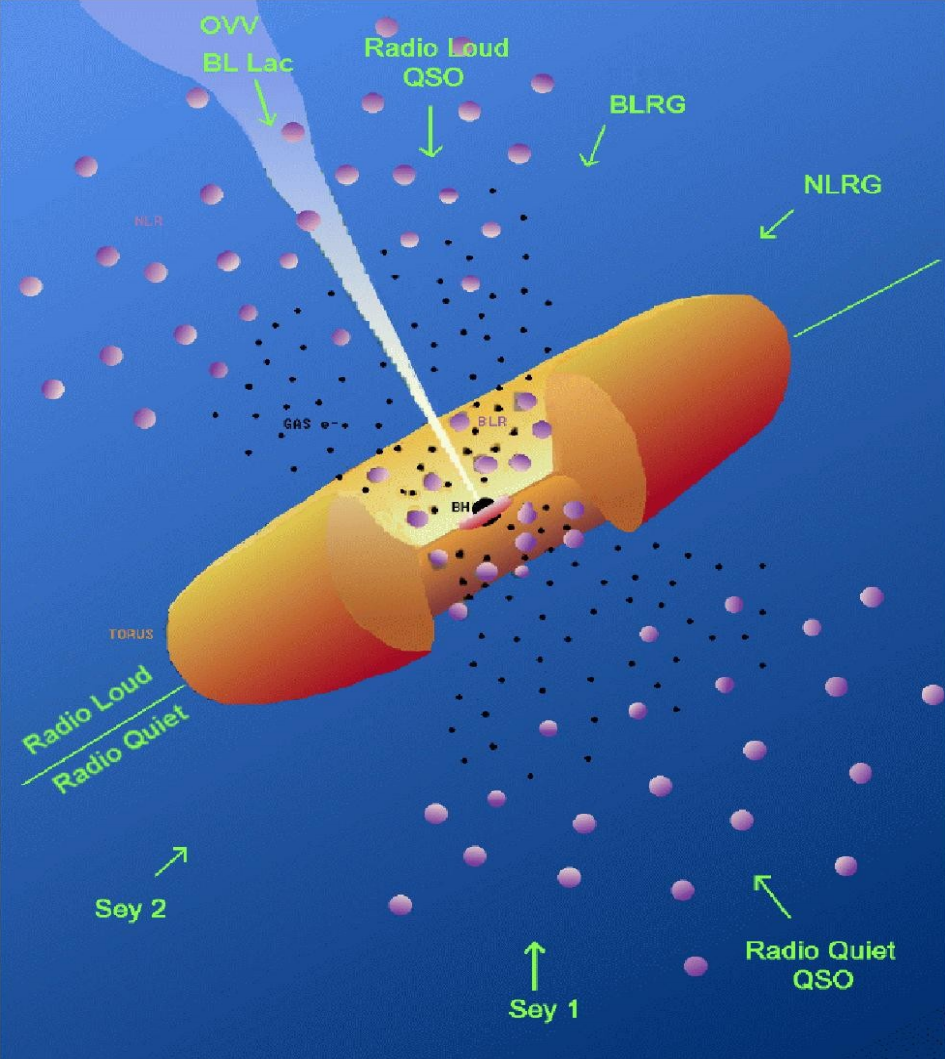
\includegraphics[width=1.0\textwidth]{figures/01-intro/up95.png}
\caption
[A unified scheme for AGN.]
{
A unified scheme for AGN.
} 
\label{fig:unification}
\end{figure} 

\nocite{elvis1994}
\begin{figure}
\centering
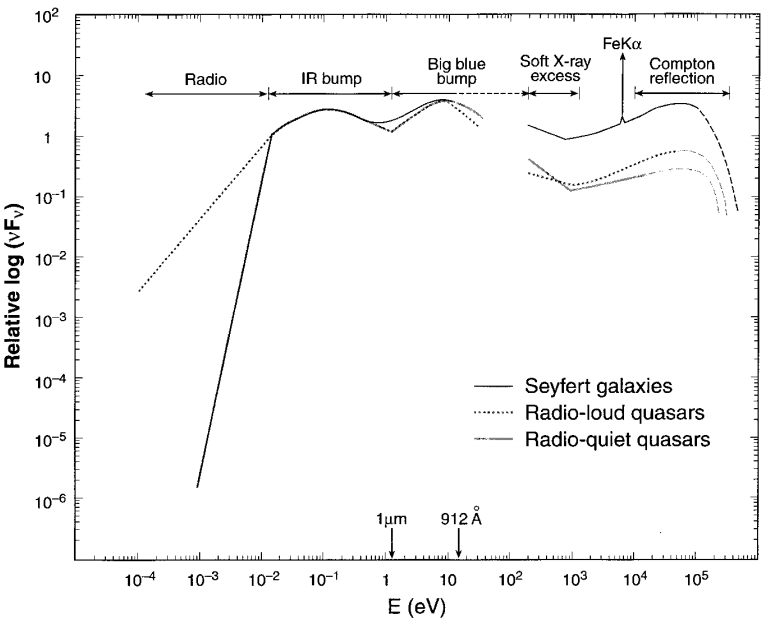
\includegraphics[width=1.0\textwidth]{figures/01-intro/agn_sed.png}
\caption
[Broadband SEDs for different AGN SEDs]
{
{\sl Credit: Koratkar \& Blaes 1999}
Approximate average broadband SEDs for a few types of AGN. The series of 
characteristic bumps can be clearly seen. 
The Soft-X-ray excess is also visible
(see section~\ref{sec:sxxs}).
} 
\label{fig:quasar_sed}
\end{figure}

Since the seminal works by AM85 and UP95, 
the picture has become somewhat more complicated. 
Variable X-ray absorption has been detected in so-called `changing look'
AGN \citep{matt2003,puccetti2007}, including even NGC 1068 itself \citep{marinucci2016}.
Changes in type have also been seen in the optical lines; 
the broad H$\beta$ component in some AGN can dramatically disappear or reappear
\citep[e.g.][]{tohline1976,cohen1986,denney2014}. 
The explanation for this could be variable absorption \citep{elitzur2012}
or a change in the accretion state of the disc. In the latter case,
it has even been suggested that a disc wind could be directly responsible
for this switch \citep{elitzur2014}.
Furthermore, dusty {\em polar} outflows
have been found to be important IR emitters \citep{hoenig2013}, implying
that, even when it comes to dust, the torus is not the whole picture.
Despite these complications, the AGN torus unification picture still
explains a lot of AGN phenomenology, and represents a useful framework 
that can be tested with observations. 


\subsection{X-ray Properties of AGN}

Approximately $10\%$ of the bolometric luminosity of AGN
comes out in the X-ray band, between $\sim0.1$ and $\sim100$~keV.
Thus, AGN dominate the cosmic X-ray background \citep{madau1994}.
The hard X-ray emission typically follows a power law shape with spectral
index -0.9 \citep[e.g.][]{koratkar1999}, 
widely considered, as in LMXBs, to come from a hot `corona' of 
electrons close to the BH that upscatters disc seed photons
\citep[e.g.][]{haardt1991}. The compactness of this X-ray corona
has been confirmed by microlensing \citep{chartas2009, dai2010} 
and variability studies \citep{green1993,crenshaw1996,risaliti2007,emmanoulopoulos2014}. 
Indeed, X-rays in AGN can be highly variable, both in terms of their intrinsic 
X-ray emission, but also due to changes in the absorption characteristics 
\citep{risaliti2002,miller2008,connolly2014}.
I discuss X-ray absorption in more detail, particularly with respect to disc winds, 
in chapter 2.

The hard X-ray spectra AGN also tend to exhibit a number of reflection features. 
Typically, these consist of a strong Fe K$\alpha$ emission line and a `Compton hump'
at high energies. The latter is produced by Compton down-scattering 
of high energy photons \citep{pounds1989,nandra1994}.
It is still unclear exactly where these features originate, 
but a common interpretation is that they are caused by 
reflection off the inner parts of the accretion disc 
\citep{fabian1995,iwasawa1996b,reynolds1999}.
If this is the case, and the broadening of the iron line is relativistic,
this would allow for measurements of the BH spin 
\citep{laor1991,iwasawa1996a,dabrowski1997}.
This hypothesis is somewhat controversial. Multiple authors have found that 
many of the relativistic features supposedly imprinted by BH spin can in fact be explained
by Comptonisation or absorption \citep[e.g.][]{misra1998,miller2013}, 
and radiative transfer modelling has shown that
an outflow can naturally produce the characteristic broad red Fe K$\alpha$ wing \citep{sim2010}.

In Compton-thick AGN, the intrinsic continuum is heavily absorbed with columns of
$N_H\sim10^{24}$~cm$^{-2}$ -- this absorption is normally attributed to the dusty torus, 
but disc winds could also contribute. Compton-thick AGN are required 
in large numbers in order to explain the cosmic X-ray background \citep{setti1989}.
In these sources, reflection features can actually dominate the X-ray spectrum 
\citep{alexander2011,gandhi2013}, but the Fe line is formed from low ionization
stages of Fe on $\sim0.1$~pc scales \citep{gandhi2015}.


\subsubsection{The Soft X-ray Excess}
\label{sec:sxxs}

If one interpolates between the $\nu^{1/3}$ law from the BBB in the UV, and the power law
in the hard X-rays, a curious excess of flux is often found
in type 1 AGN \citep[see figure~\ref{fig:quasar_sed}, and][]{koratkar1999}. 
This is known as the soft X-ray excess (SXXS), which is too 
hot to be explained by thermal disc emission, as a thin disc around an AGN should
never approach the temperatures required. Many models have been proposed to
explain this excess, including relativistically smeared 
photoabsorption \citep{gierlinskidone2004b,gierlinskidone2006}, 
relativistically smeared line and free-free emission \citep{rossfabian2005} 
and a variety of cool Comptonised component geometries such as an 
inner accretion flow \citep{magdiarz1998,done2012} 
and thin layer on top of the disc \citep{januik2001}. 
While the SXXS poses a challenge to
the simplest pictures of AGN, it may also solve some of the issues, as
some of the geometries proposed may help to explain the 
accretion disc size problem discussed in 
section~\ref{sec:disc_continuum} \citep{gardnerdone2016}.

\subsection{The Broad Line Region: Connection to winds and unification}

In the UP95 unification model, the broad emission lines
come from a series of virialised clouds close to the disc plane.
As noted by \citet[][hereafter MCGV95]{MCGV95}, there are a number of problems with
the BLR `cloud' model, perhaps most notably that there is no obvious 
physical origin for such virialised clouds. 
Testing alternative models for the BLR is therefore important.
Indeed, MCGV95 proposed a disc wind model in order to explain both BALs and BELs
in quasars. A disc wind model was also  discussed by \cite{elvis2000}, 
who proposed a structure for quasars that attempted to explain much 
of the behaviour of luminous AGN
merely as a function of viewing angle. Outflow models are discussed further in section~2.
The philosophy of these models is that, before invoking additional
degrees of freedom in a model, we should first test if known quasar phenomenology 
(disc winds) can explain other aspects of their observational appearance.
I have illustrated this general principle with the `Occam's quasar' 
cartoon shown in figure~\ref{fig:occam}. This is the picture that I will
quantitatively test in the latter, quasar-focused sections of this thesis.
The same general principle can also be applied to cataclysmic variables 
and other accreting objects.


\begin{figure}
\centering
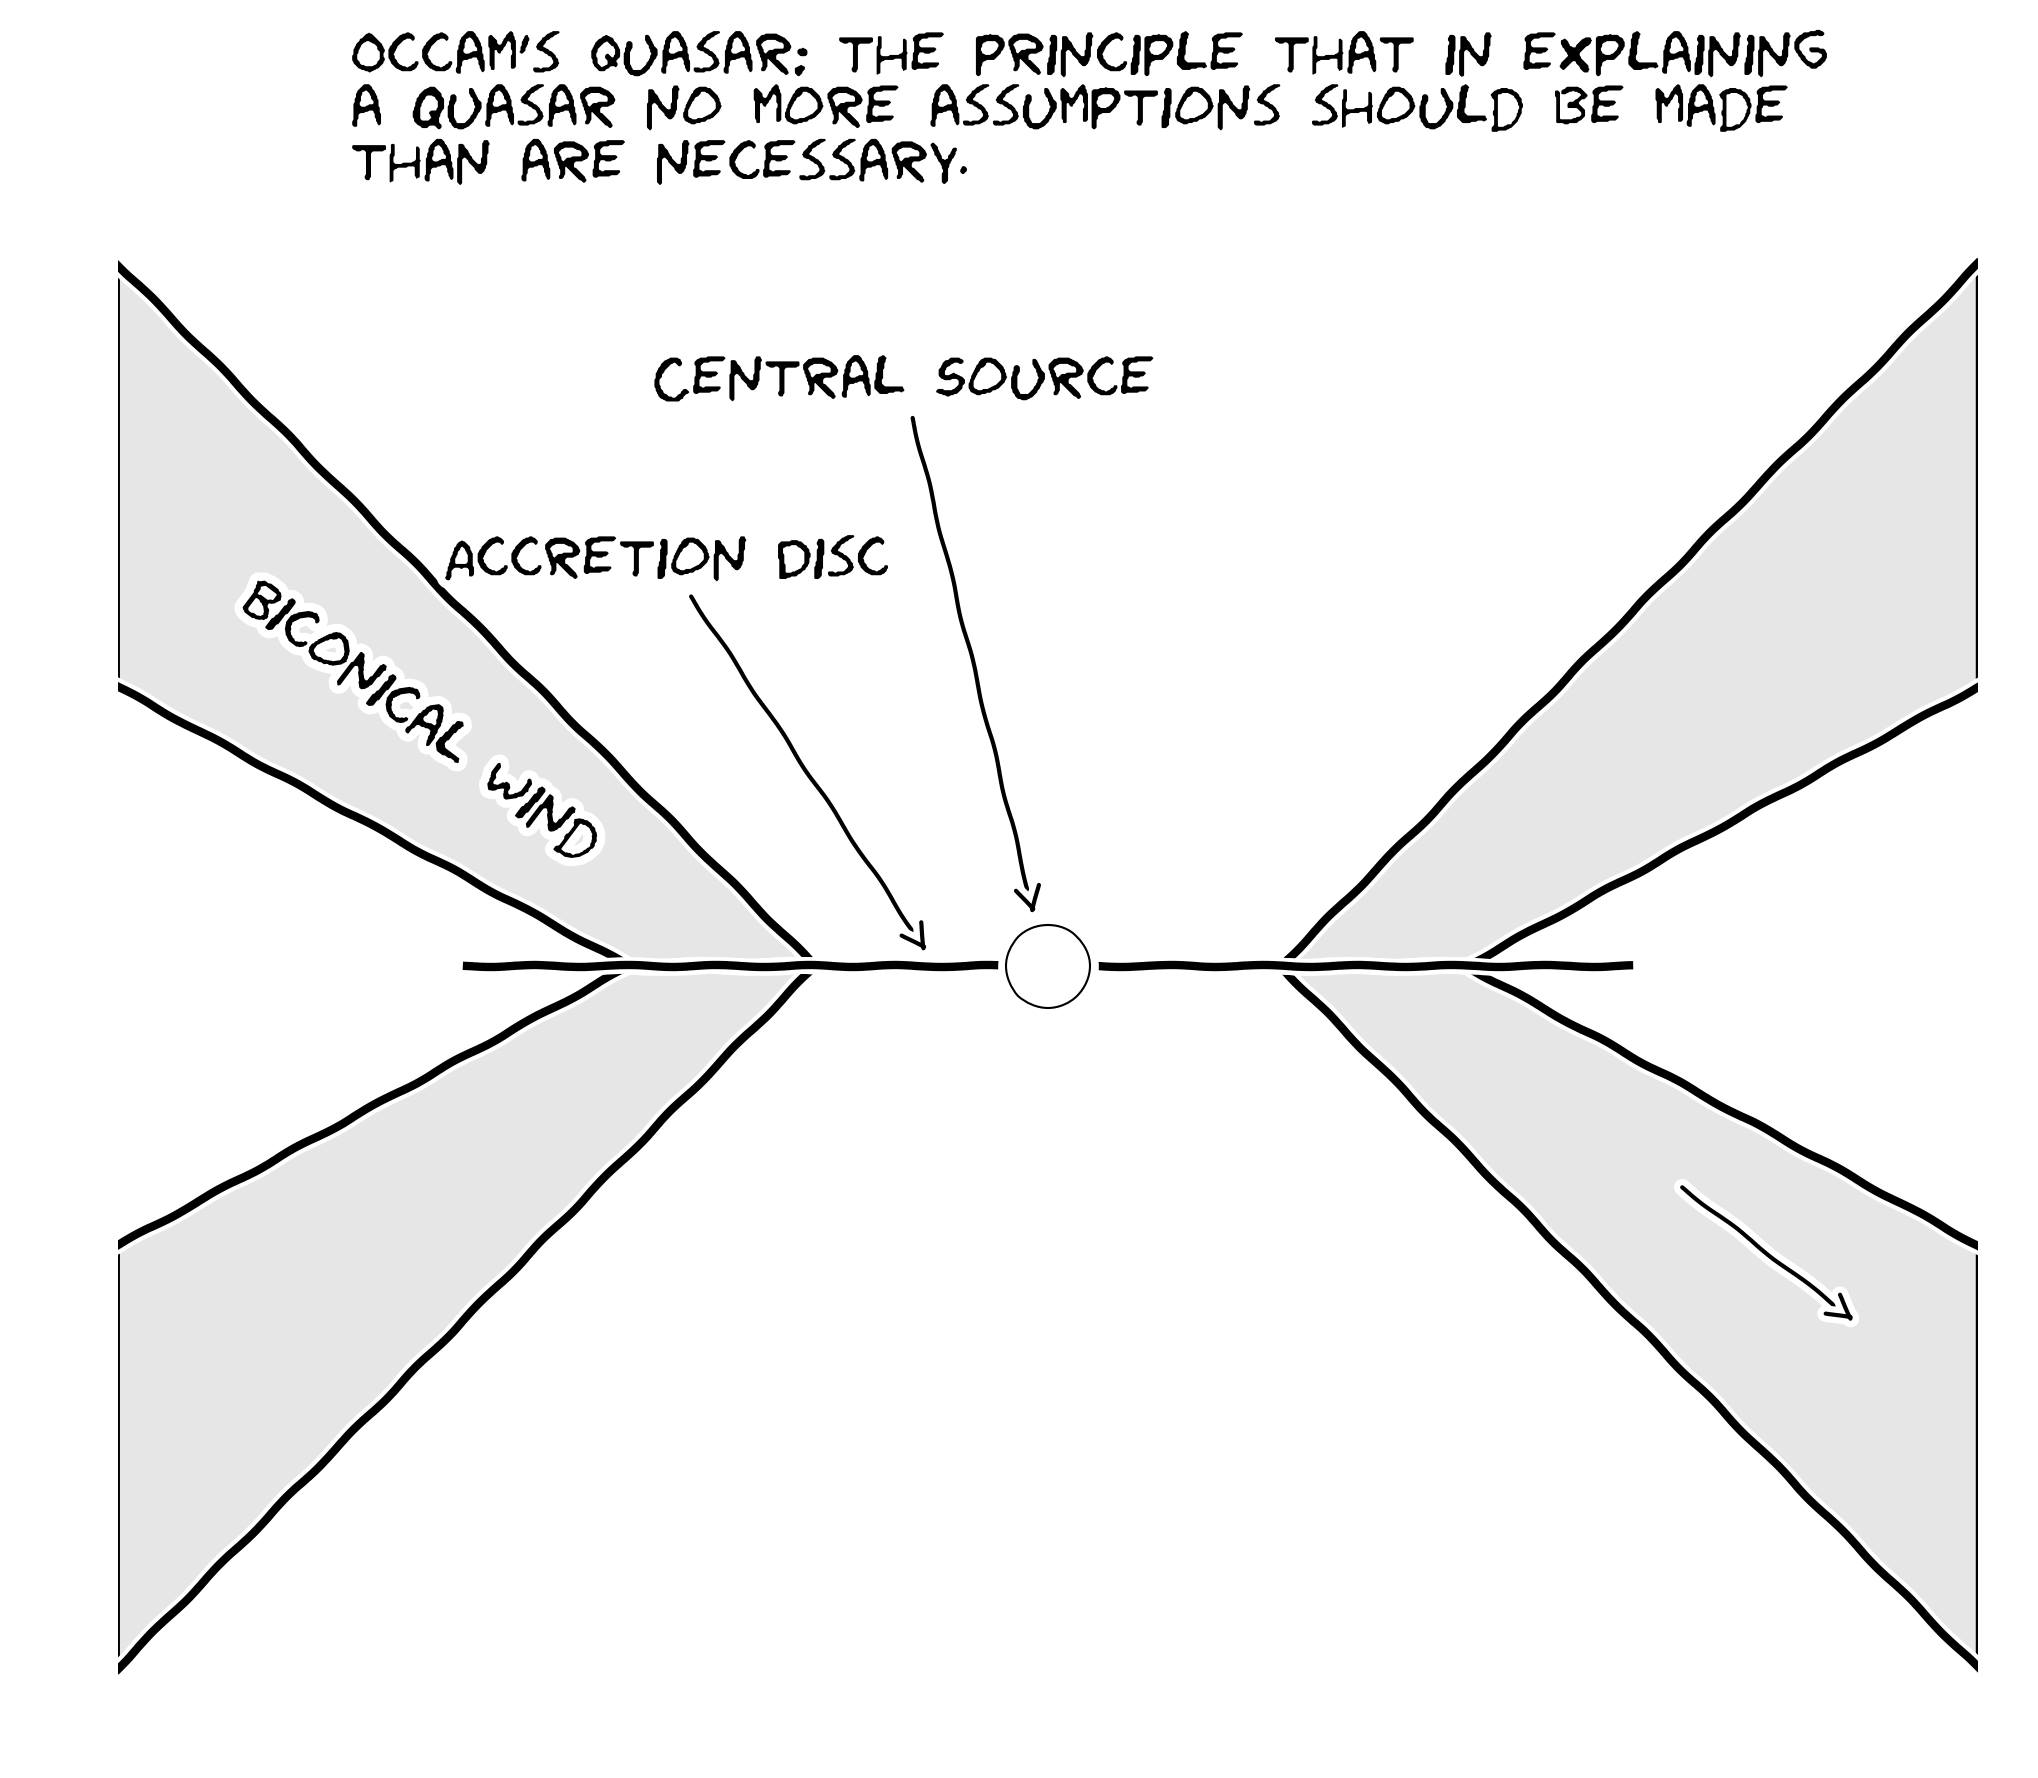
\includegraphics[width=1.0\textwidth]{figures/01-intro/occam.jpg}
\caption
[Occam's quasar]
{
Occam's quasar. How far can this general picture take us when trying to explain
the behaviour of quasars and other accreting compact objects?
} 
\label{fig:occam}
\end{figure}


\section{The Current Understanding of the Disc Continuum}

\label{sec:disc_continuum}

The SS73 model is still the most common way to fit accretion disc spectra and infer
information about the underlying physics. However, 
a number of issues have been raised with the thin-disc model and
its applicability to accreting systems. 

\subsection{The Spectral shape of CV discs}

Attempts to fit the observed SEDs of high-state CVs with simple disc models 
have met with mixed success. In
particular, the SEDs predicted by most stellar/disc atmosphere models 
are too blue in the UV \citep{wade1988,long1991,long1994,knigge1998} and exhibit
stronger-than-observed Balmer jumps in absorption 
\citep{wade1984,haug1987,ladous1989b,knigge1998}. One possible
explanation for these problems is that these models fail to capture
all of the relevant physics. Indeed, it has been argued that a
self-consistent treatment can produce better agreement with 
observational data (e.g. Shaviv et al. 1991;  but see also Idan et al. 2010).
\nocite{idanshaviv2010} \nocite{shaviv1991}
However, an alternative explanation, suggested by Knigge et al.
(1998b; see also Hassall et al. 1985)\nocite{KLWB98,hassall}, 
is that recombination continuum emission from the base of the 
disc wind might fill in the disc's Balmer absorption edge and flatten 
the UV spectrum.

Alternatively, it may just be that CV disks are never really in
a steady state, and so we should only expect the $R^{-3/4}$
temperature profile to hold in a limited portion of the disc.
From eclipse mapping, it has been shown that the inferred accretion
rate increases with radius in NLs \citep{rutten1992, horne1993}.
These results suggest that a non-radiative form of energy loss
is present in the inner regions of the disc, of which potential forms
would be advection or mass loss. This is yet another piece of evidence
that the understanding of accretion and outflow 
are intertwined, although hopefully not inextricably.

\subsection{The Big Blue Bump in AGN}

Does the SS73 model apply well to AGN spectra? There are constrasting views on the matter.
On the one hand, \cite{antonucci2013} claims that ``most of the AGN community is mesmerized by unphysical models that have no predictive power''. 
Yet a recent spectral fitting study by \cite{capellupo2015} concludes that 
``altogether, these results indicate that thin ADs are indeed the 
main power houses of AGN''. So, what are the current problems when 
confronting thin disc models with observation? 

\subsubsection{The Accretion Disc Size Problem}

One of the most interesting results of recent years relating to AGN and accretion discs is
the discovery that the continuum emission region size appears to be
a factor $\sim3$ larger than predicted by standard thin disc theory. This result
has been found independently in both microlensing \citep{morgan2010,dai2010} 
and reverberation \citep{edelson2015} studies, and poses a challenge to the 
current best-bet model for the big blue bump in AGN. 
One proposed solution is that the discs in AGN are inhomogenous,
consisting of individual clumps with independently
varying temperatures \citep{dexteragol2011}, but this is very much
still an active area of research. It is worth noting that the impact
of winds on these results has not yet been properly quantified, something
our team is currently trying to address \citep{mangham}.

\subsubsection{Fitting AGN Spectra and the 1000\AA\ Break}

One of the {\em successes} of the thin disc model, when applied to AGN,
is that we do observe a slope in the UV of $\alpha_{UV} = 0.32$, confirming
the theoretical prediction of $\nu^{1/3}$. 
However, AGN spectra do not exhibit the {\em overall} spectral shape 
\citep[e.g.][]{davis2007,shankar2016} or colour-mass scalings \citep{bonning2007} 
expected from theoretical predictions. 
This can be seen clearly in figure~\ref{fig:agn_templates},
where both the quasar and Seyfert spectra tend to peak in the UV, rather than
the EUV. Furthermore, there is a characteristic break in AGN spectra at
around $1000$~\AA\ \citep{lusso2015}, which does not scale with BH mass or luminosity,
as one might expect for a break associated with an accretion disc. 
There is also no evidence in AGN of the expected polarisation signatures from an 
optically thick disc atmosphere \citep{stockman1979,antonucci1988,antonucci1996}. 

Despite these problems, recent work suggests that the thin disc model 
still has some potential. \cite{capellupo2015} were able to fit a number of
AGN spectra in the UV and optical with thin disc models, although successful fits
were only found once they included effects such as Comptonisation and mass-loss,
as well as correcting for extinction. BH spin also had a reasonable effect on the 
spectral fits, although it is somewhat difficult to constrain from spectral fitting alone.
The $1000$~\AA\ break has also been explained with a mass-losing disc \citep{laordavis2014},
and \cite{lusso2015} suggested that incorrect IGM corrections 
may be exacerbating the effect.
So, while many problems exist, it may not quite be time to 
abandon the Shakura-Sunyaev ship just yet.

\section{The Universality of Accretion}

Accretion appears to be an important physical processes across $\sim10$ orders
of magnitude in mass. But is this process the same on all scales? Does any 
behaviour manifest in all accreting systems? 

\subsection{The RMS-flux relation}

Broad-band variability is common in all types of accretion disc. It has been
known for some time that there exists a linear relationship
between the flux and absolute root-mean-square (rms) amplitude
of this variability. This was discovered first in XRBs and AGN 
\citep{uttley2001, uttley2005, heil2012}, but it has been shown
more recently that the relationship extends to CVs and even YSOs 
\citep{scaringi2012,scaringi2015a}. The relationship is also not limited
to just one type of CV but is present in both NLs and DNe \citep{vandesande2015}.
 
The model that best reproduces this behaviour is the so-called
`fluctuating accretion disc' model \citep{lyubarskii1997,kotov2001,
arevalo2006,hogg2015}. More generally,
additive processes cannot reproduce this behaviour, and a multiplicative
mechanism is required \citep{uttley2005}. 
Regardless of the mechanism, the rms-flux relation is one of the most
clear-cut examples of a universal accretion phenomenon. 
It tells us that at least some of the behaviour in CV discs
is also present in AGN and XRBs, strengthening the argument that CVs
can be used as `accretion laboratories'. 


\subsection{Accretion states and disc-jet coupling}
\label{sec:disc-jet}

Variable and transient sources are common in astrophysics, particularly
when the sources are accreting. I have already mentioned the DIM an
and its applicability to LMXBs and CVs; it turns out that when one plots
the colour and luminosity evolution over the course of an ourburst cycle 
then they follow very similar tracks \
citep[see figure~\ref{fig:kording_hid}, ][]{kordingDNjet2008}.
The detection of radio jets is also intrinsically linked to the accretion state
of the system (disc-jet coupling), as jets only appear in the `hard' accretion 
state, to the right of the so-called `jet line' \citep{fender2001,fender2004}.
\cite{kordingDNjet2008} showed that this behaviour also occurs in CVs, 
as radio emission in the DN SS Cyg is also detected in the same region 
of colour-luminosity space. There is also a well-known correlation between 
radio and X-ray luminosities in low-hard states \citep{gallo2003}.

This clear correlation with accretion state on HIDs has natural parallels 
with AGN. 


The jet production mechanism in BHs in general is not well known. 
Theoretical work suggests that radio jets should be correlated with BH spin 
\citep{penrose1971,blandford1977}, 
but whether such a correlation exists in LMXBs is 
controversial \citep{fender2010,narayan2012}.
This has significant implications for AGN; if powerful radio jets are 
associated exclusively with rotating BHs then the number of radio-loud AGN
would imply a large fraction of them must be rapidly spinning, with
high radiative efficiencies. 
Further evidence that radio jets are not simply produced by RIAFs onto spinning
BHs is found when one considers that NLs show evidence of synchrotron
radio emission \citep{coppejans2015}. This important result suggests that our understanding
of jets is incomplete, and that the links between accretion state and 
jet production are fundamental, but unsolved. Disc winds may complicate, or simplify,
matters, depending on one's outlook (see chapter 2).

\begin{figure}
\centering
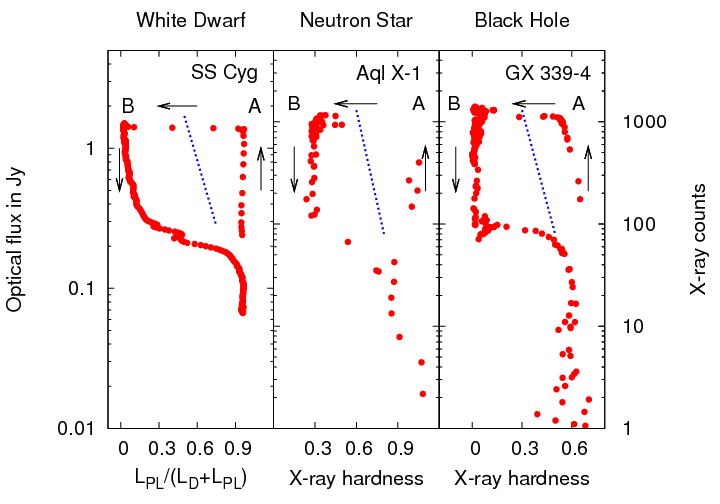
\includegraphics[width=1.0\textwidth]{figures/01-intro/kording_hid.png}
\caption
[Hardness-intensity diagrams for three types of accreting objects.]
{
{\sl Credit: Kording et al. 2008.} 
Caption.
} 
\label{fig:kording_hid}
\end{figure}

\subsection{A Global Picture}

Clearly, accretion physics is relevant to a plethora of astrophysical phenomena, 
and at least some of the physics of accretion is applicable to {\em all} 
classes of accreting object. 
It would also appear that the outflowing material observed in accreting systems 
has a profound effect on the accretion process itself, and 
possibly significantly affects the observational 
appearance of disc-accreting systems (c.f. Elvis unification model). 
Hence, in the next chapter, I will review the evidence for
winds and discuss some of the relevant background theory.

